%%%%%%%%%%%%%%%%%%%%%%%%%%%%%%%%%%%%%%%%%%%%%%%%%%%%%
\chapter{Combination of searches for diboson resonances at $\sqrt{s}$ = 8 and 13 TeV}
\label{ch:combination}
%%%%%%%%%%%%%%%%%%%%%%%%%%%%%%%%%%%%%%%%%%%%%%%%%%%%%

%%%%%%%%
\section{Inputs to the combination}

\subsection{8 TeV VV searches}
\subsection{13 TeV VV searches}
\subsection{8 TeV VH searches}
\subsection{13 TeV VH searches}

%%%%%%%%
\section{Combination procedure}

%%%%%%%%
\section{Results}

\subsection{Limits on W'}

\begin{figure}[htbp]
\centering
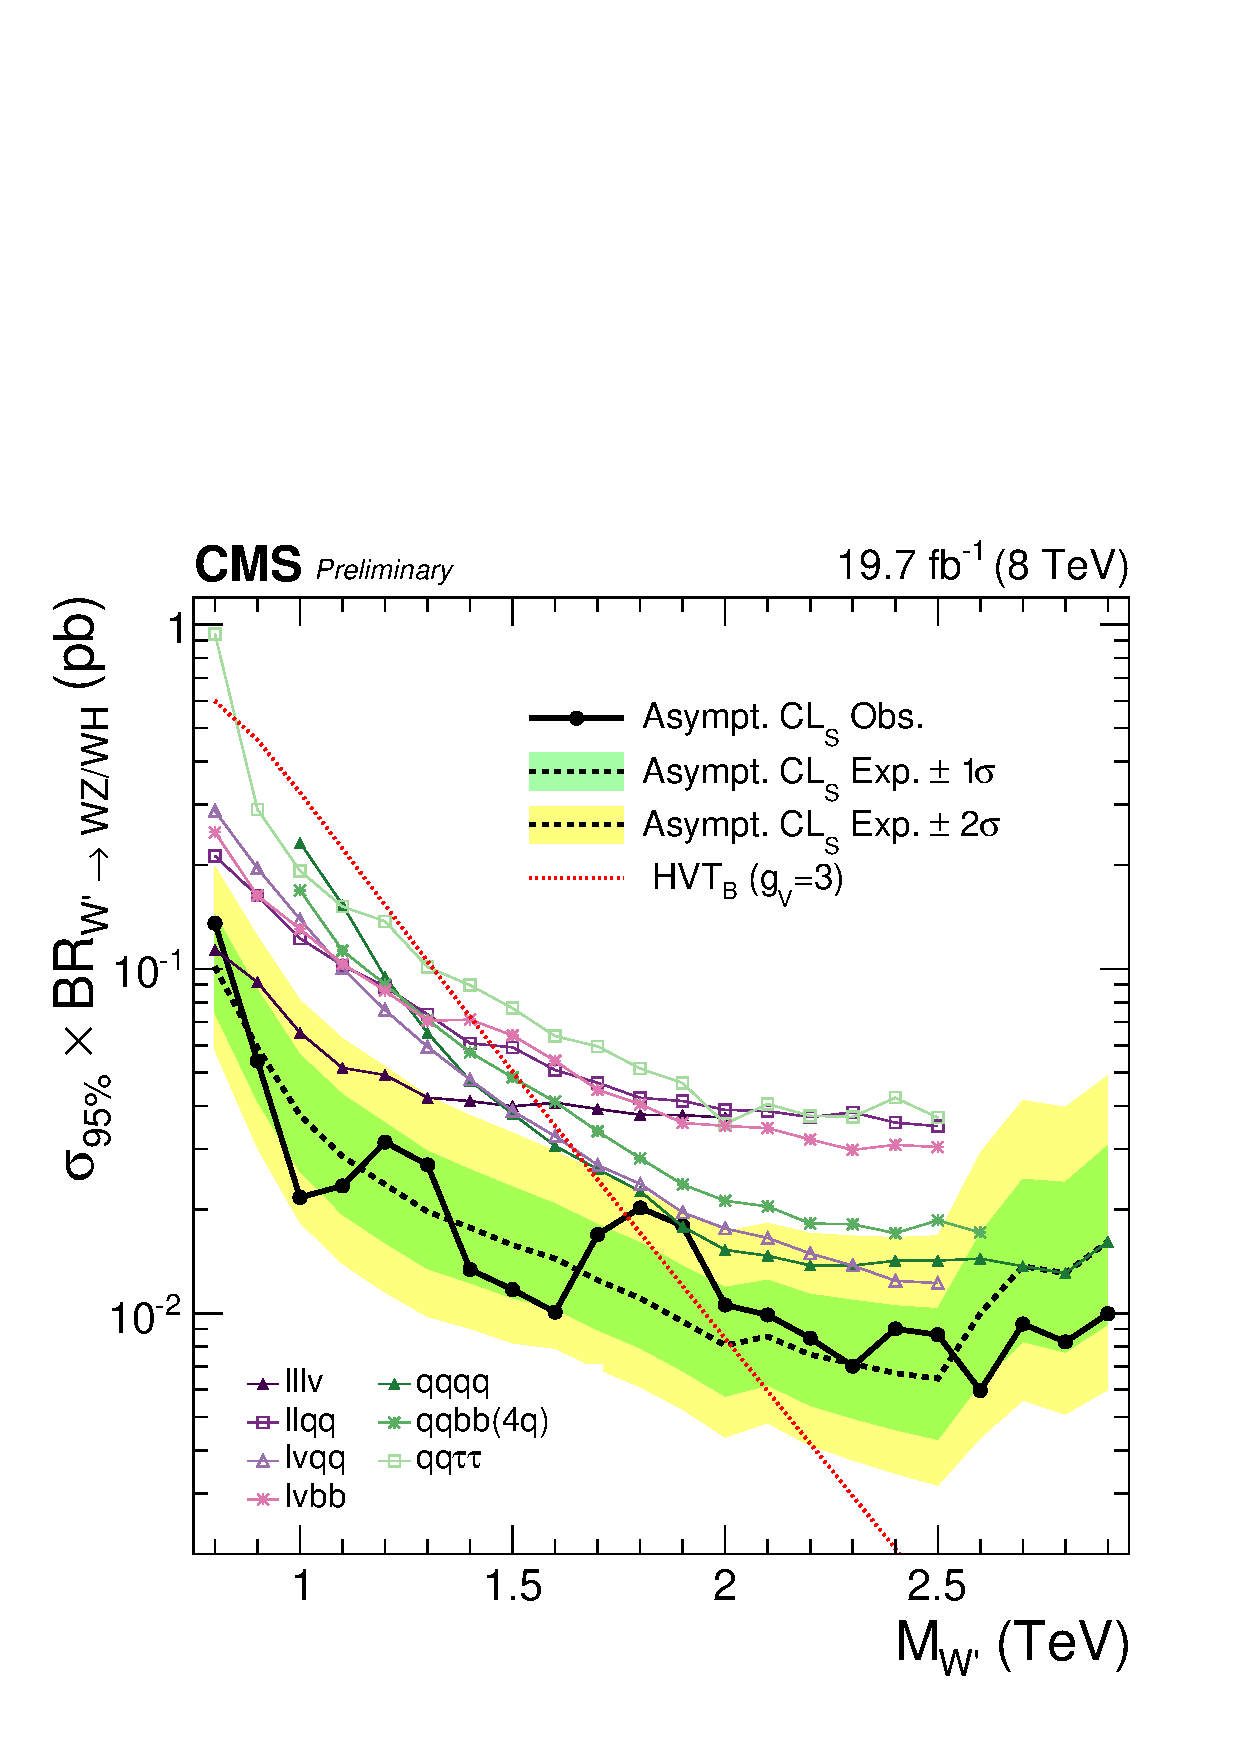
\includegraphics[width=0.48\textwidth]{\chthirteen/EXOVVhvt_compare_ALLWPRIME8_final.pdf}
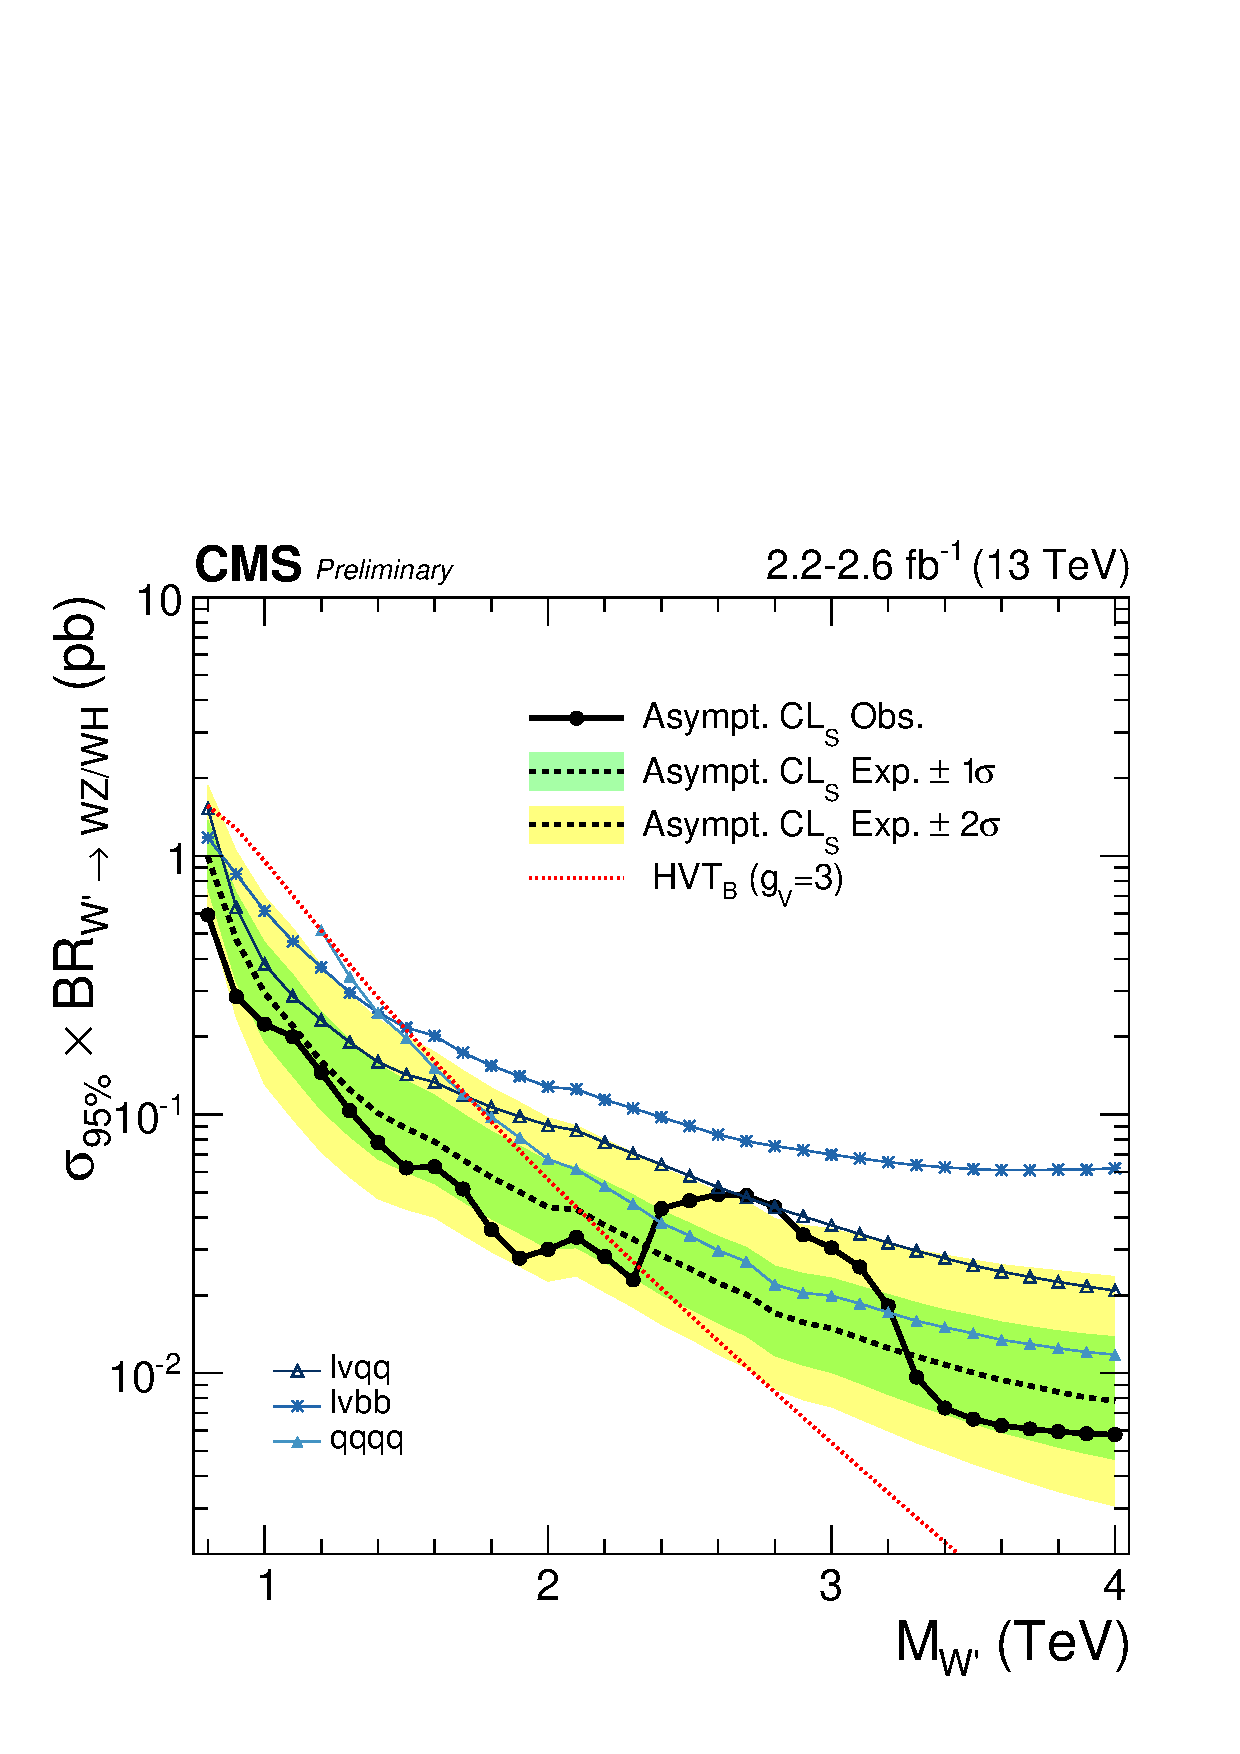
\includegraphics[width=0.48\textwidth]{\chthirteen/EXOVVhvt_compare_ALLWPRIME13_final.pdf}
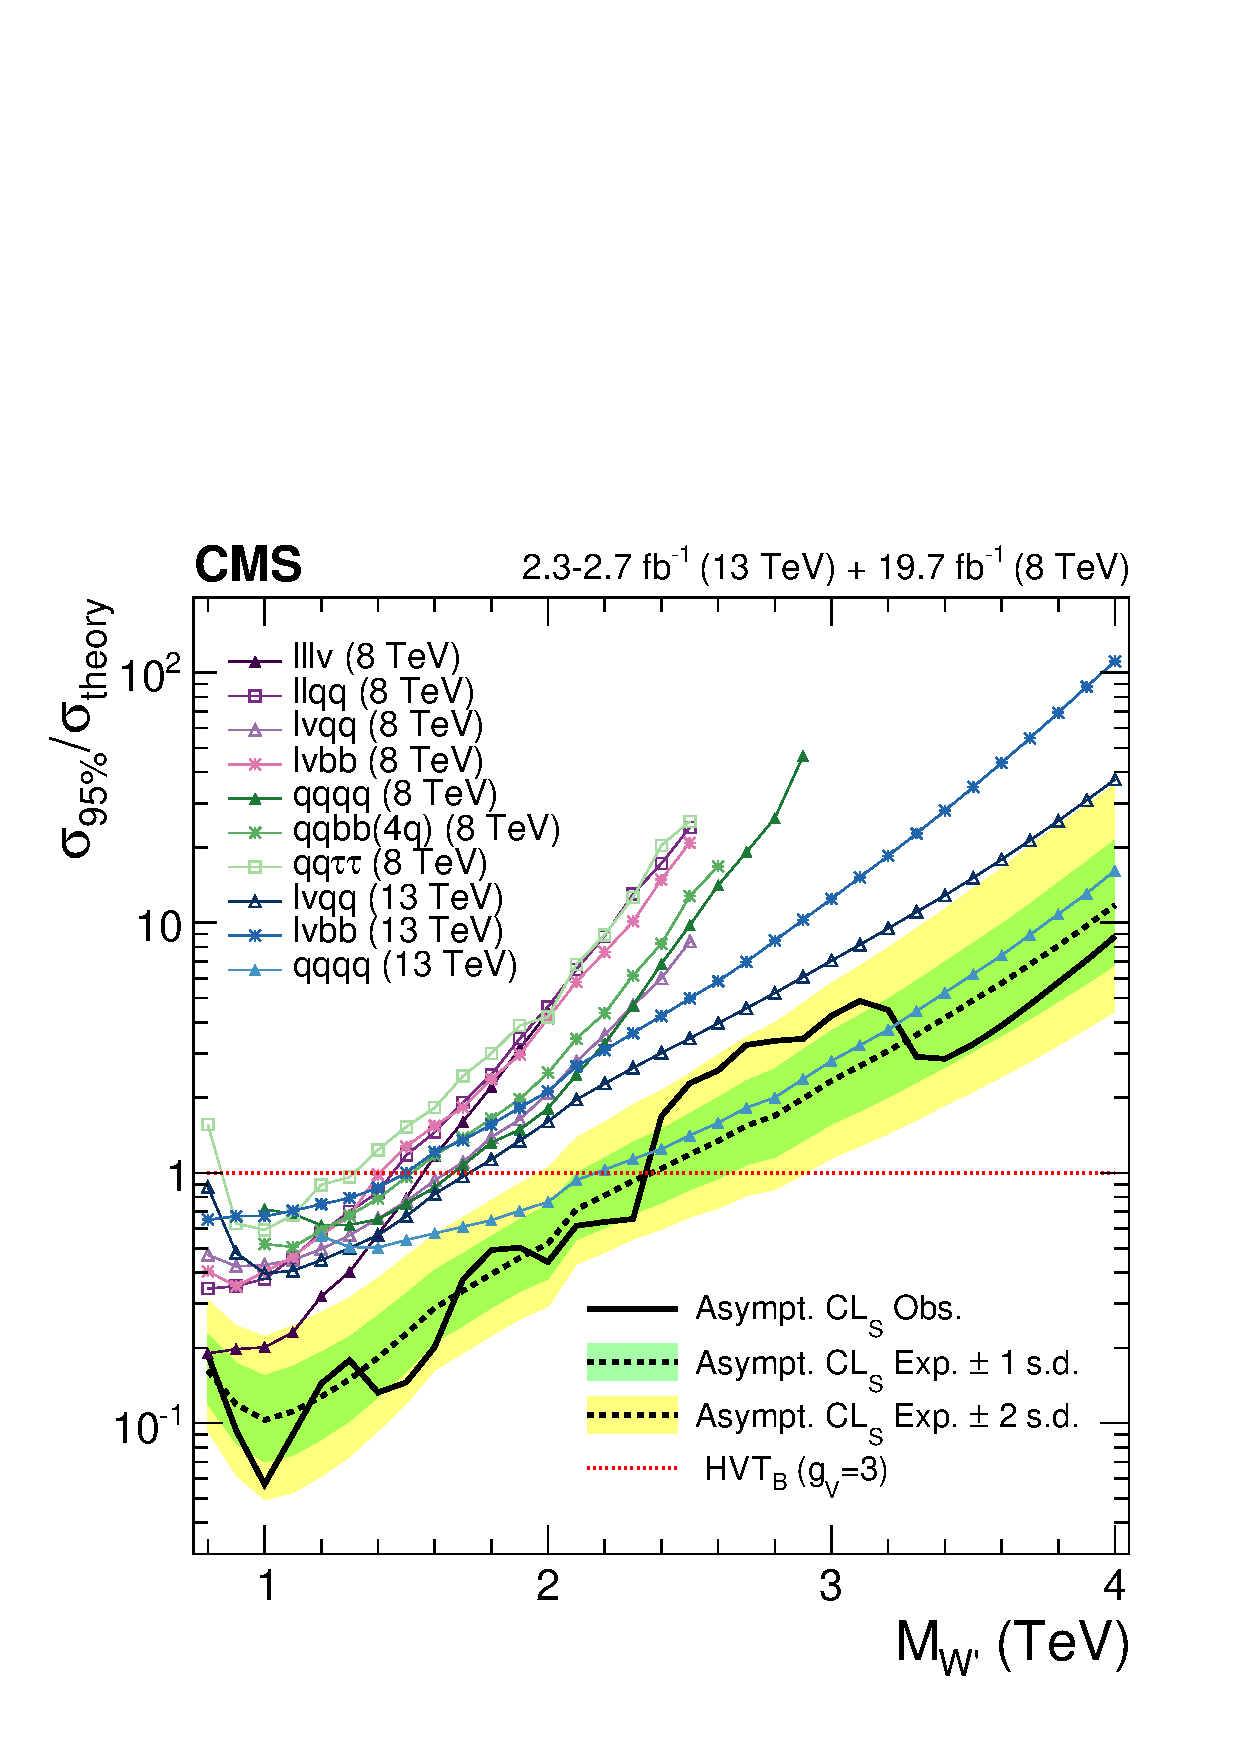
\includegraphics[width=0.48\textwidth]{\chthirteen/EXOVVhvt_compare_ALLWPRIME138_final.pdf}
\caption{%
(top left) Observed (black solid) and expected (black dashed) exclusion limits at 95\% CL on $\sigma( \rm pp \to \PWpr \to WZ/WH)$ as a function of the resonance mass obtained by combining the 8 TeV diboson searches. The curve corresponding to the cross sections predicted by the HVT model B is overlaid. (top right) Observed (black solid) and expected (black dashed) exclusion limits at 95\% CL on $\sigma( \rm pp \to \PWpr \to WZ/WH)$ as a function of the resonance mass obtained by combining the 13 TeV diboson searches. The curve corresponding to the cross sections predicted by the HVT model B is overlaid. (bottom) Exclusion limits at 95\% CL on the signal strength as a function of the resonance mass obtained by combining the 8 and 13 TeV diboson searches. In each of the three plots the different colored lines correspond to the searches entering the combination.}
\label{fig:wpall_138TeV}
\end{figure}

\begin{figure}[htbp]
\centering
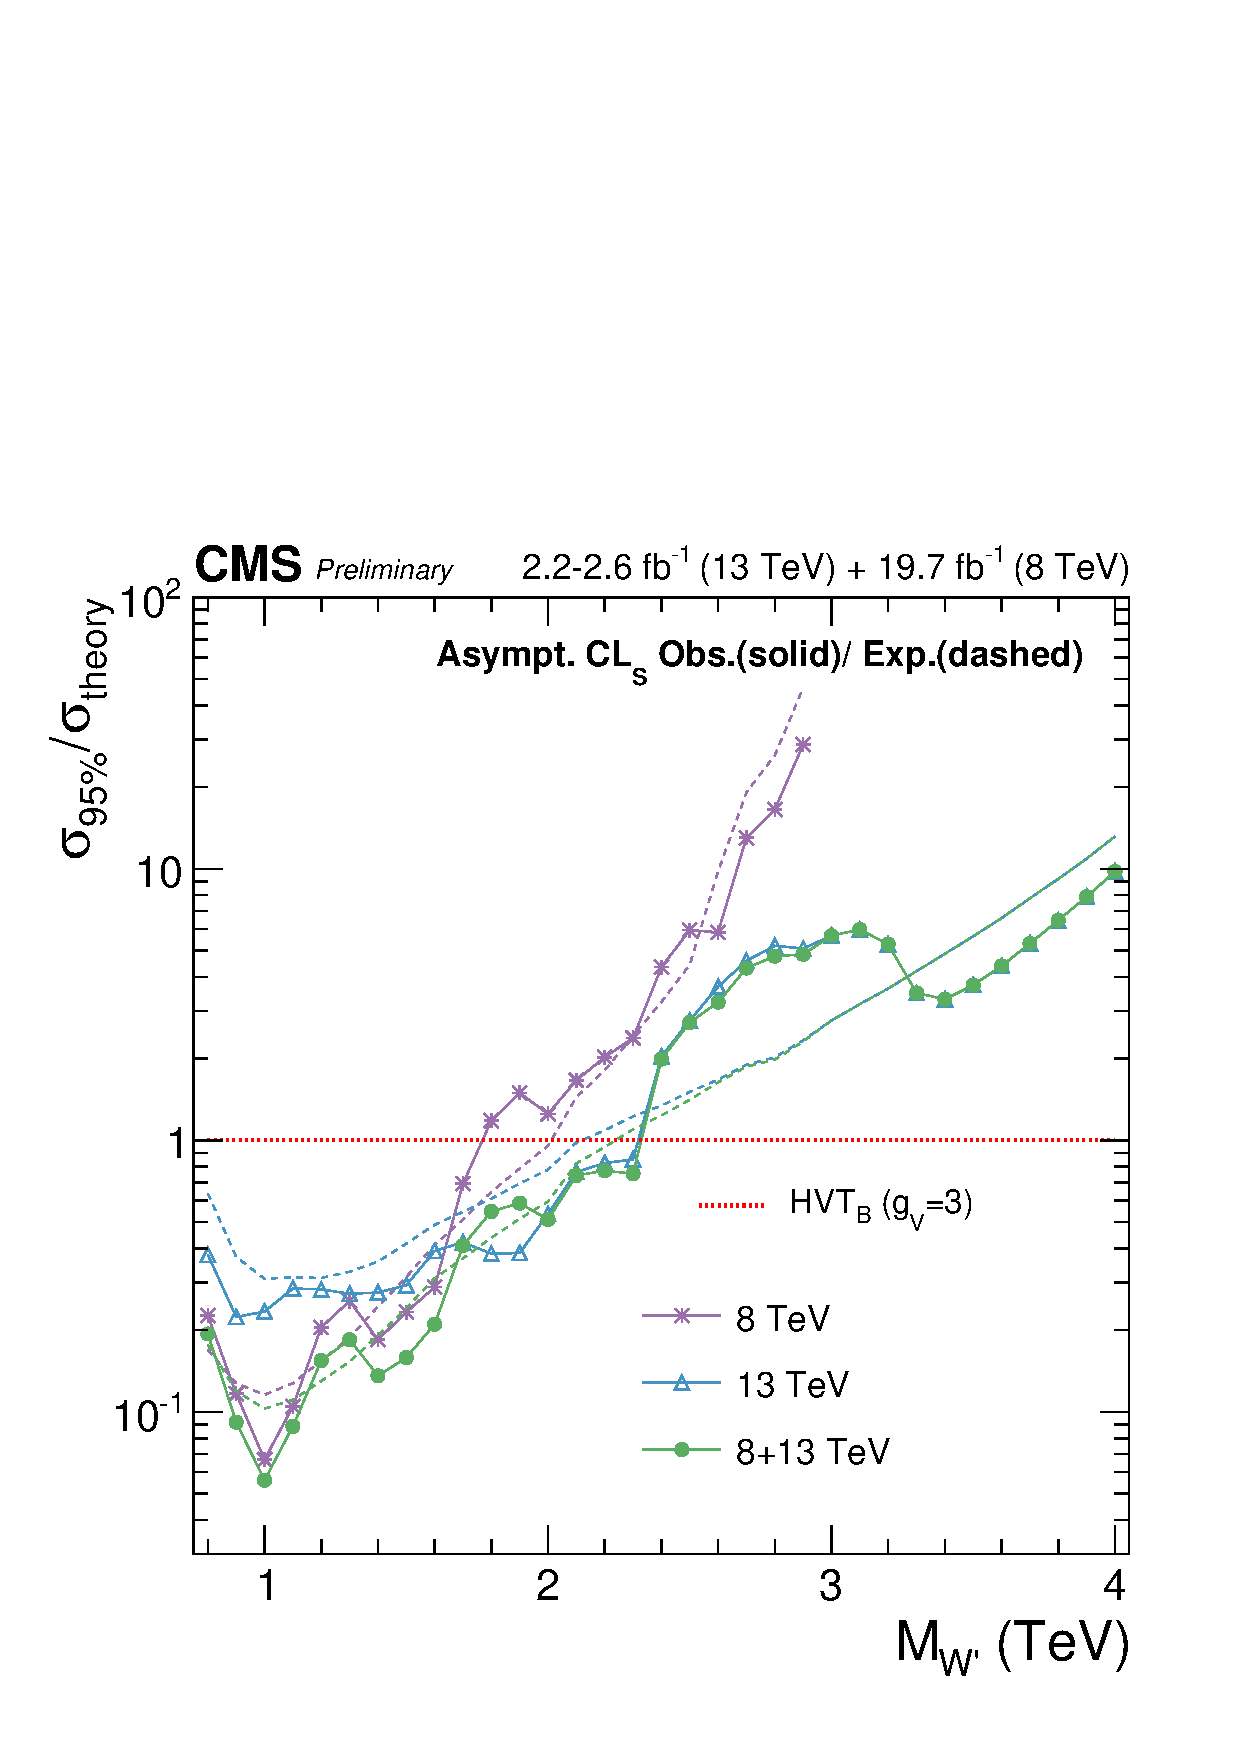
\includegraphics[width=0.48\textwidth]{\chthirteen/EXOVVhvt_compare_ALLWPRIME_expected.pdf}
\caption{%
Comparison of the observed (solid) and expected (dashed) exclusion limits at 95\% CL obtained by combining only 8 TeV or only 13 TeV searches to the results from the combination of all the 8 and 13 TeV results.}
\label{fig:wpall_compare}
\end{figure}

\subsection{Limits on Z'}

\begin{figure}[htbp]
\centering
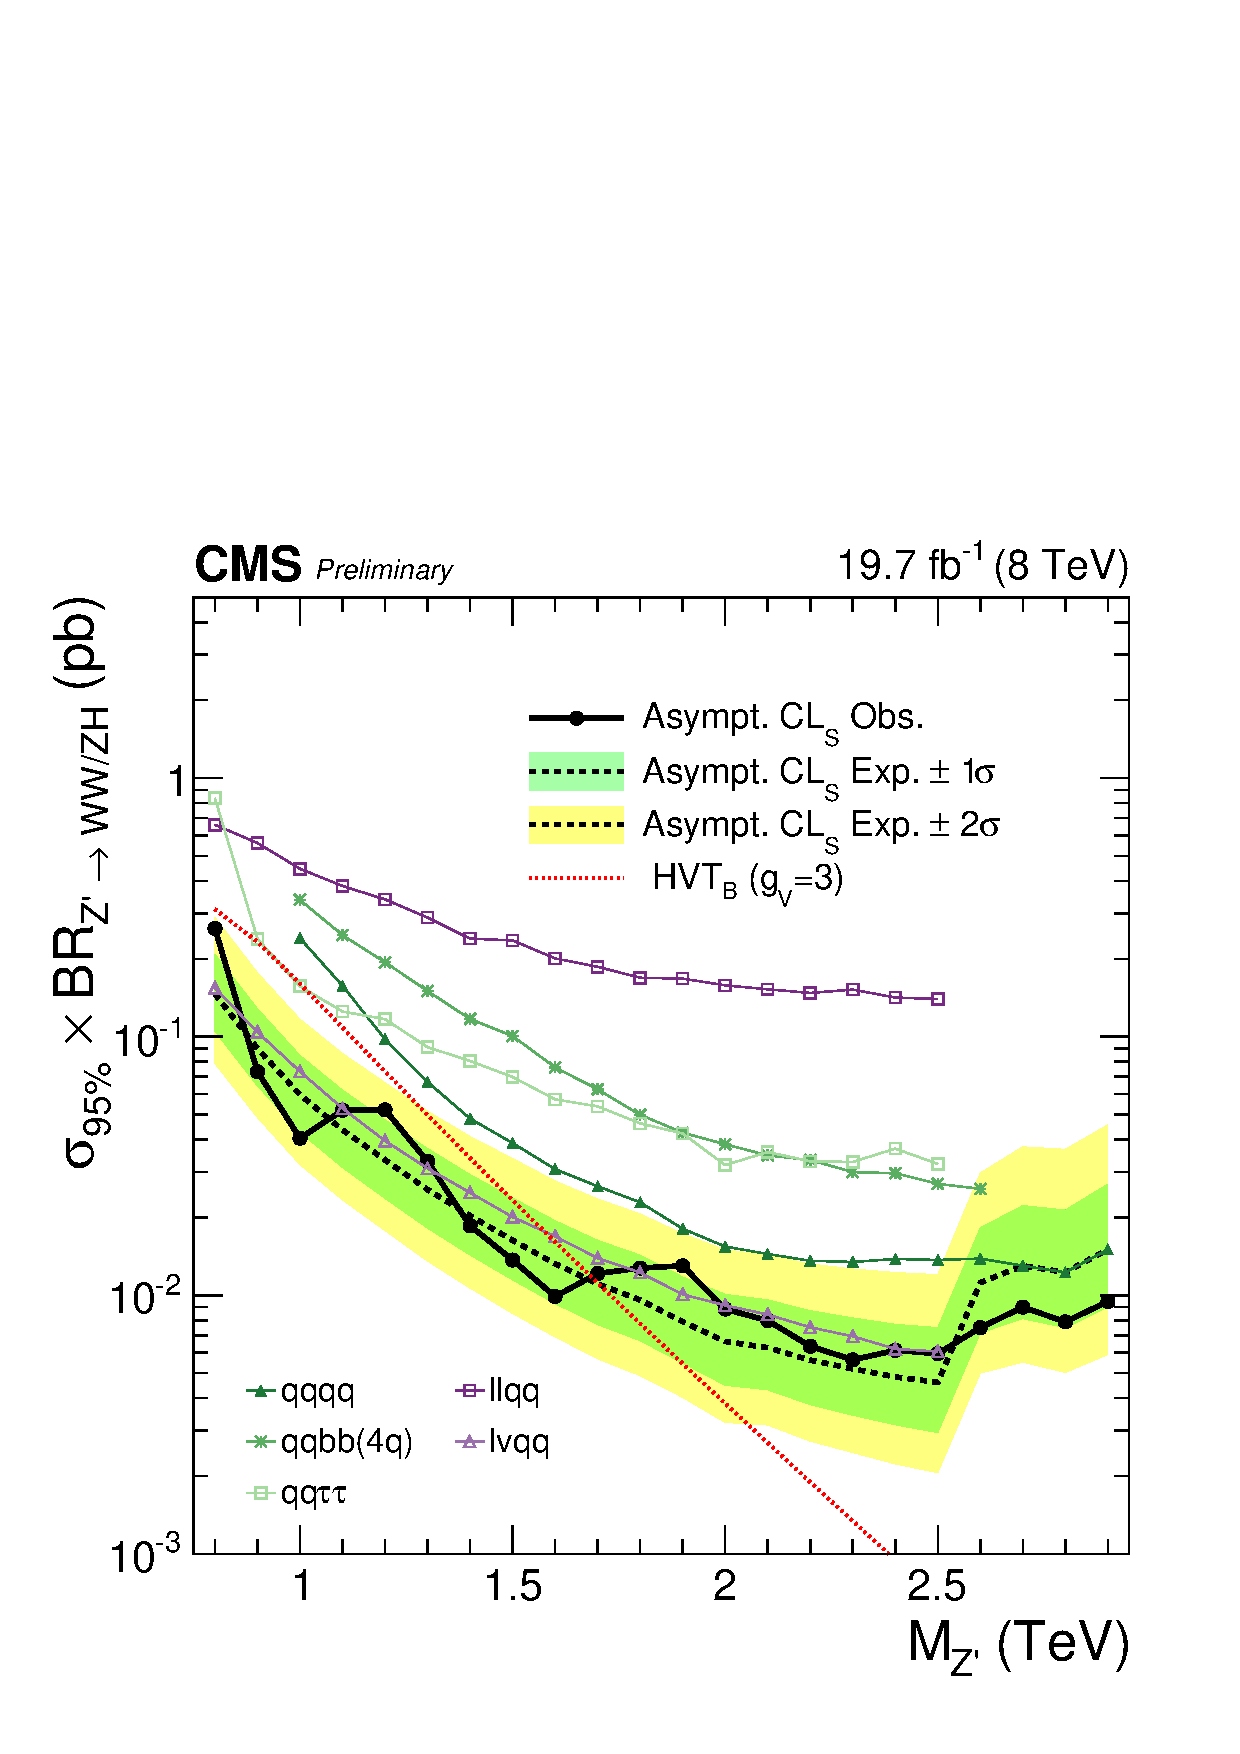
\includegraphics[width=0.48\textwidth]{\chthirteen/EXOVVhvt_compare_ALLZPRIME8_final.pdf}
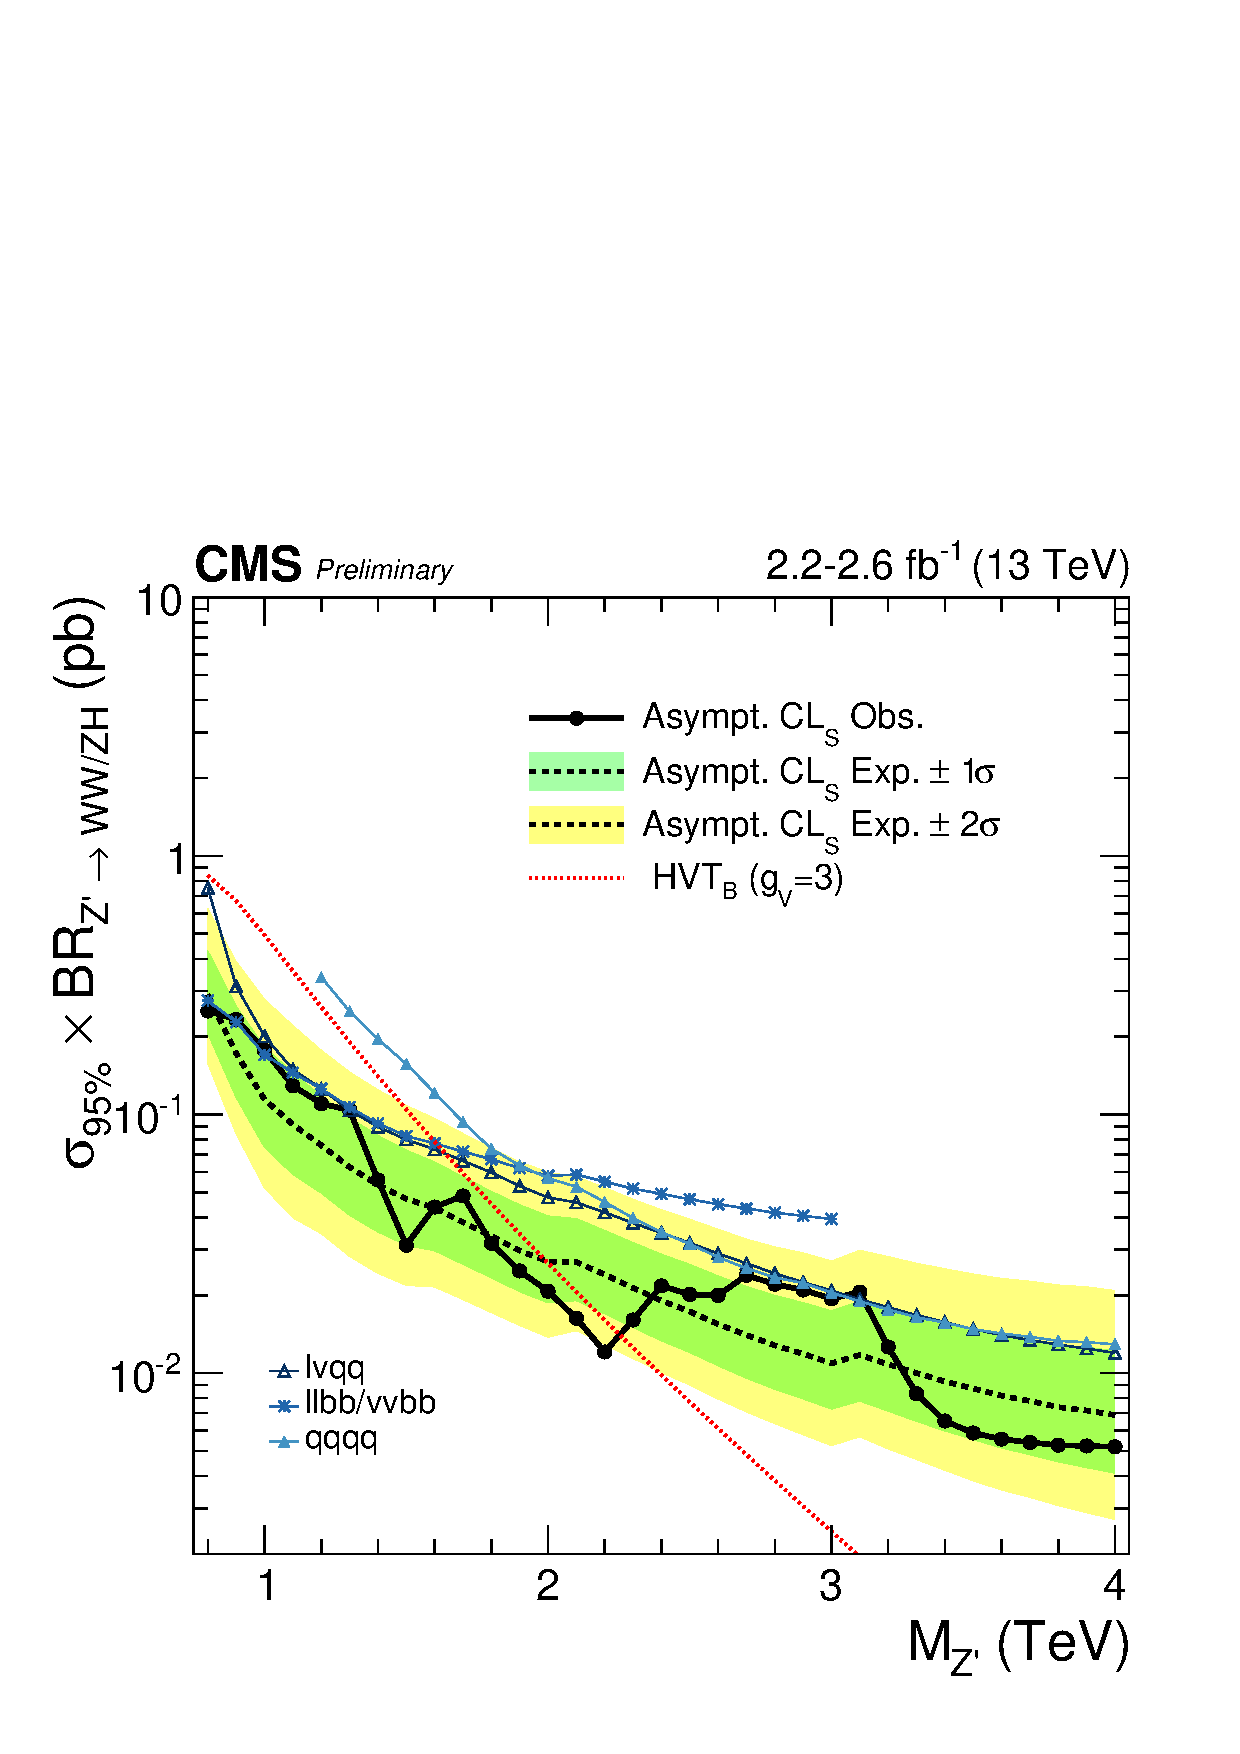
\includegraphics[width=0.48\textwidth]{\chthirteen/EXOVVhvt_compare_ALLZPRIME13_final.pdf} \\
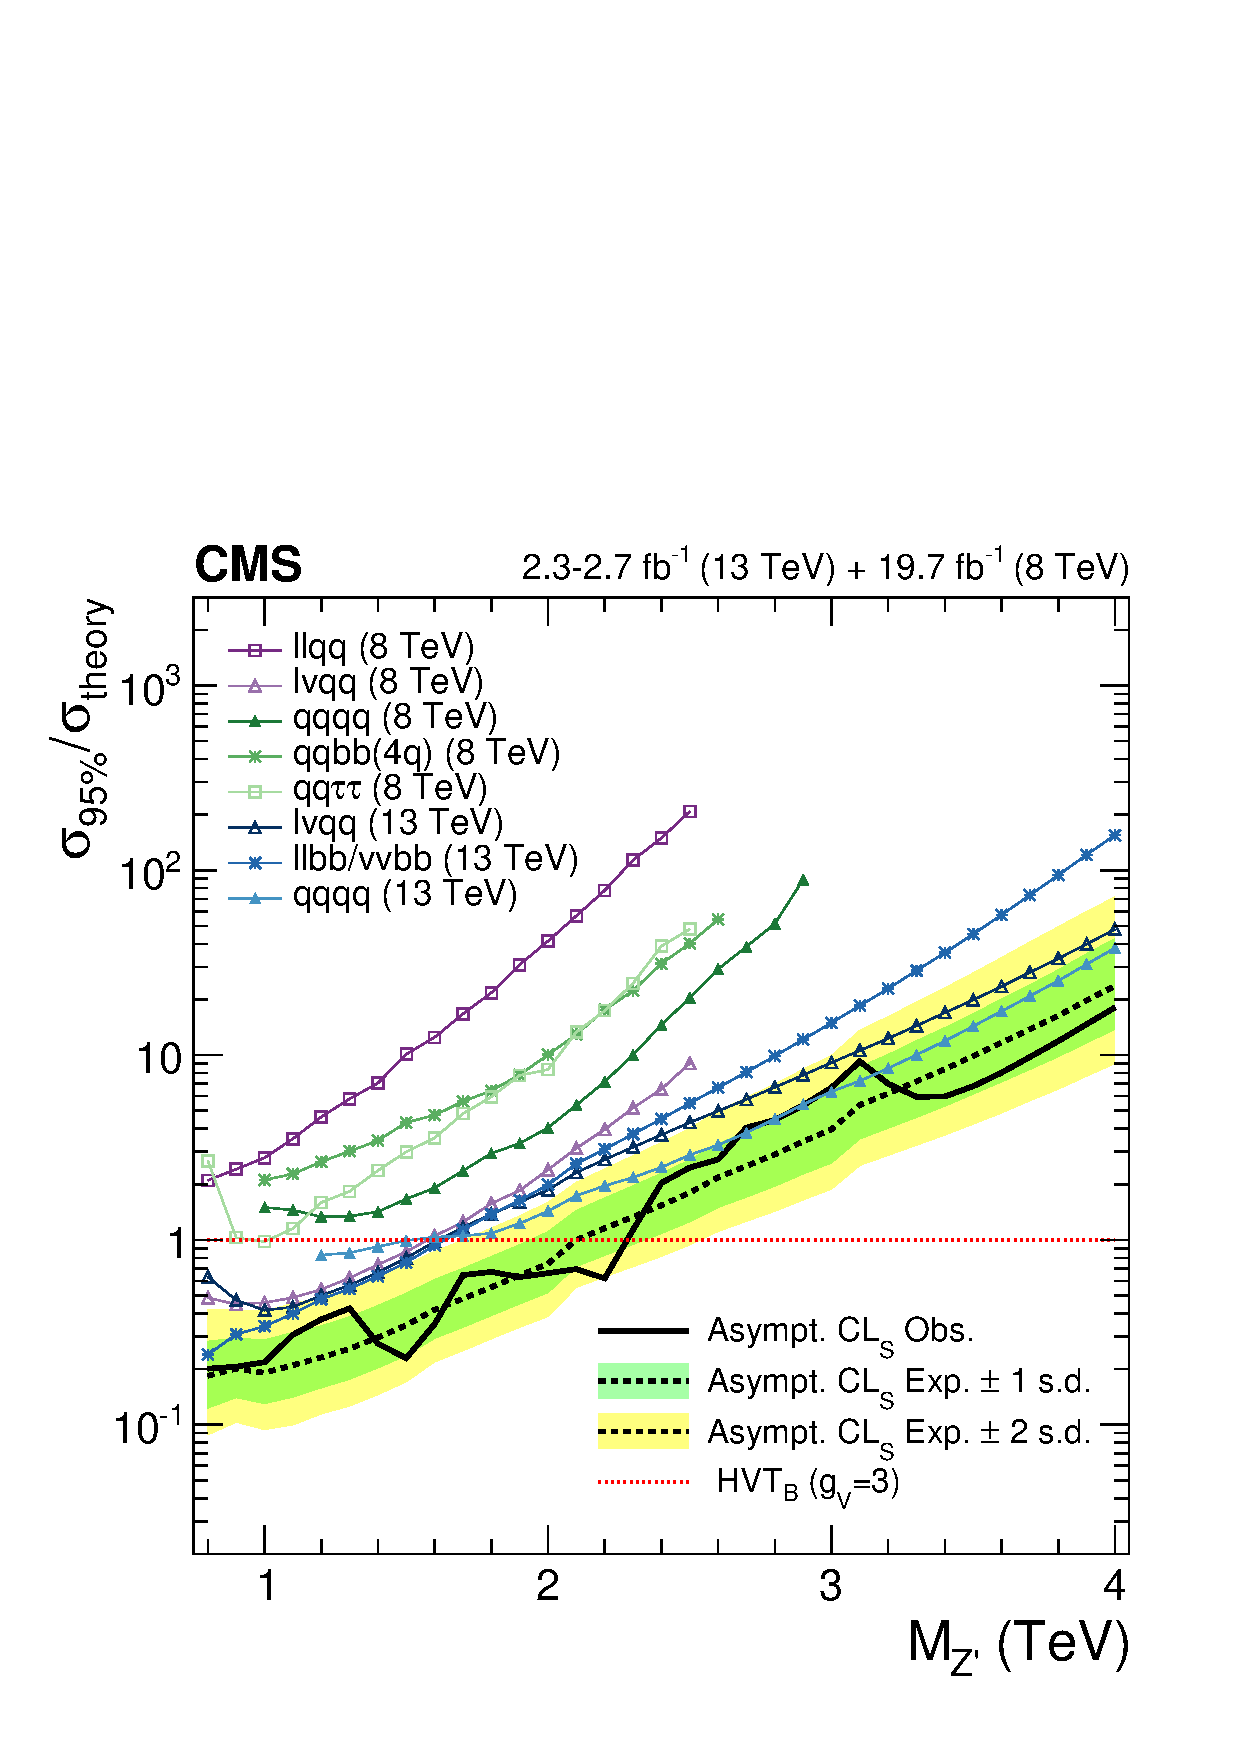
\includegraphics[width=0.48\textwidth]{\chthirteen/EXOVVhvt_compare_ALLZPRIME138_final.pdf}
\caption{%
(top left) Observed (black solid) and expected (black dashed) exclusion limits at 95\% CL on $\sigma( \rm pp \to \PZpr \to WW/ZH)$ as a function of the resonance mass obtained by combining the 8 TeV diboson searches. The curve corresponding to the cross sections predicted by the HVT model B is overlaid. (top right) Observed (black solid) and expected (black dashed) exclusion limits at 95\% CL on $\sigma( \rm pp \to \PZpr \to WW/ZH)$ as a function of the resonance mass obtained by combining the 13 TeV diboson searches. The curve corresponding to the cross sections predicted by the HVT model B is overlaid. (bottom) Exclusion limits at 95\% CL on the signal strength as a function of the resonance mass obtained by combining the 8 and 13 TeV diboson searches. In each of the three plots the different colored lines correspond to the searches entering the combination.
}
\label{fig:zpall_138TeV}
\end{figure}

\begin{figure}[htbp]
\centering
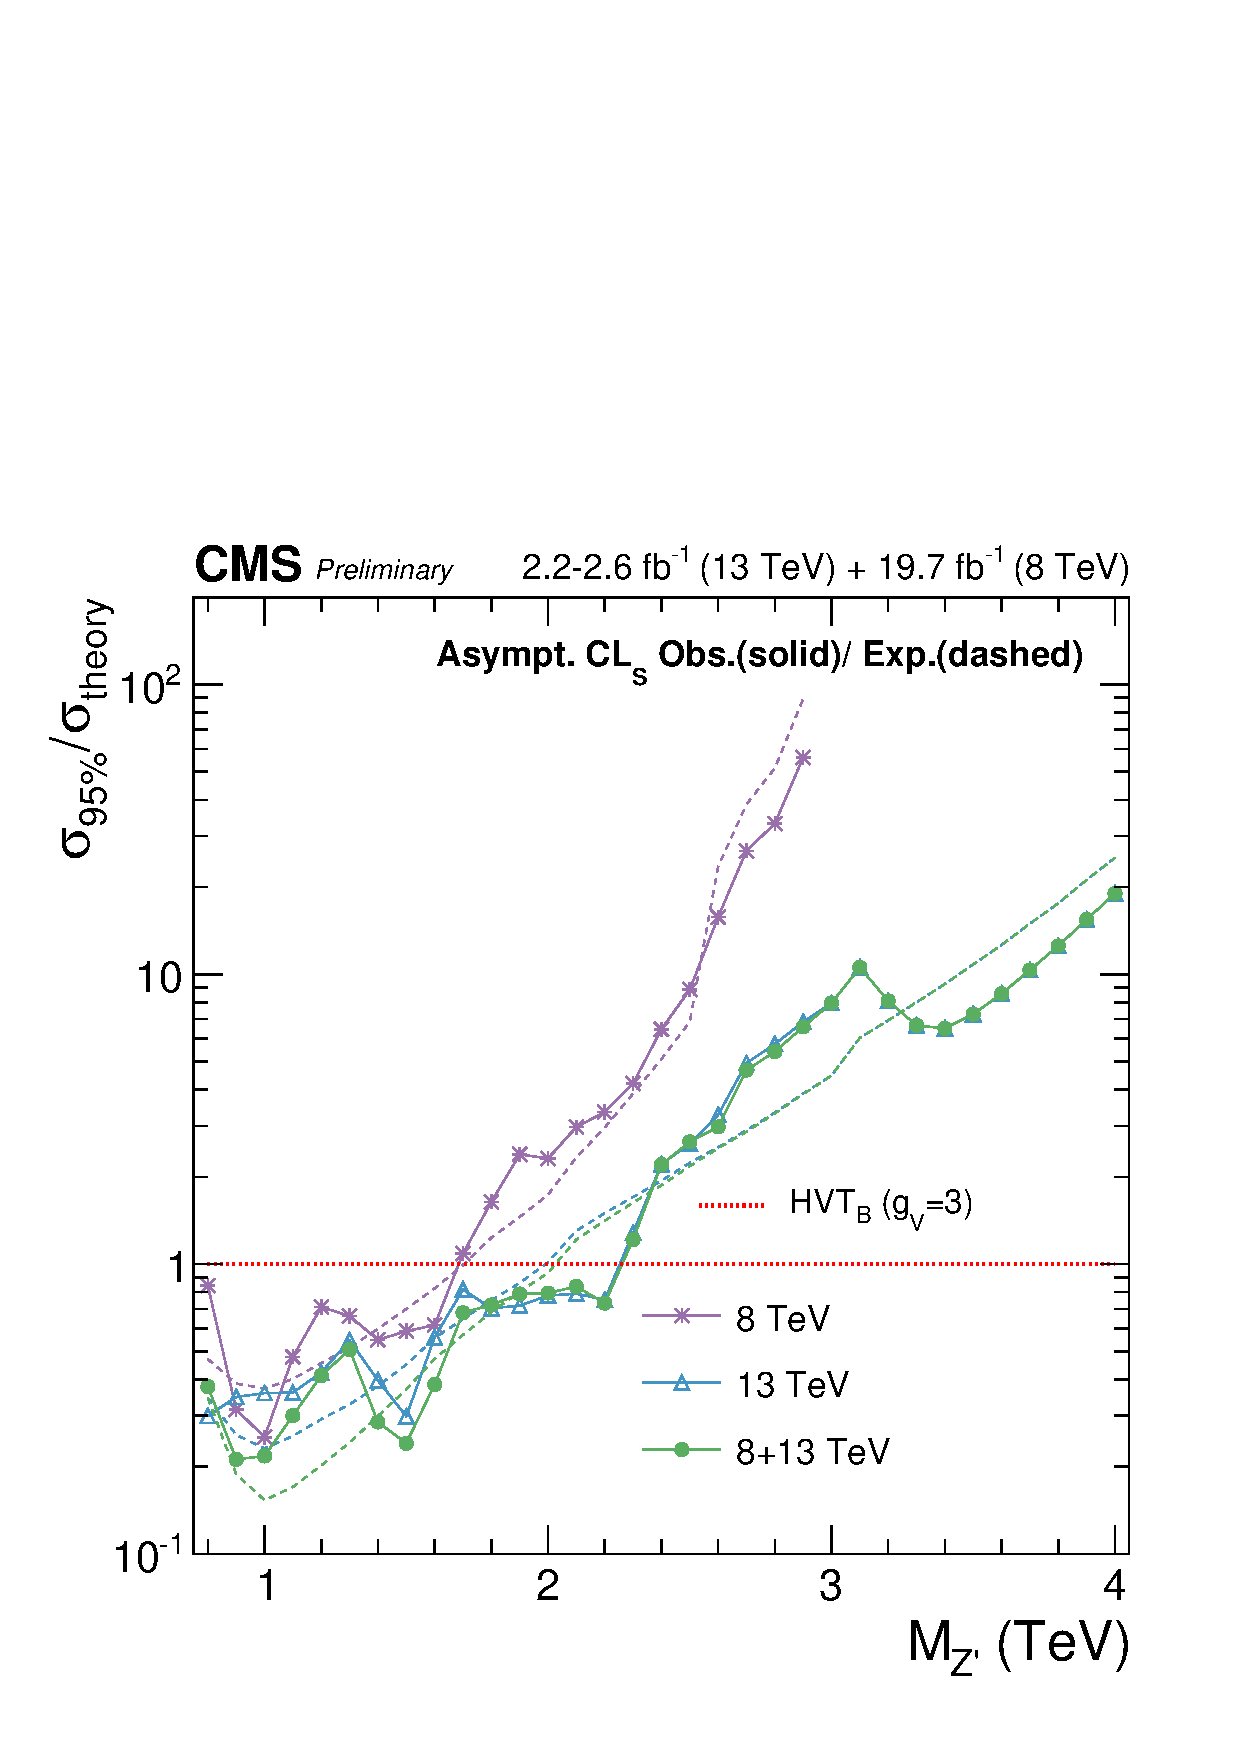
\includegraphics[width=0.48\textwidth]{\chthirteen/EXOVVhvt_compare_ALLZPRIME_expected.pdf}
\caption{%
Comparison of the observed (solid) and expected (dashed) exclusion limits at 95\% CL obtained by combining only 8 TeV or only 13 TeV searches to the results from the combination of all the 8 and 13 TeV results.}
\label{fig:zpall_compare}
\end{figure}

\subsection{Limits on heavy vector triplet (W'+Z')}

\begin{figure}[htbp]
\centering
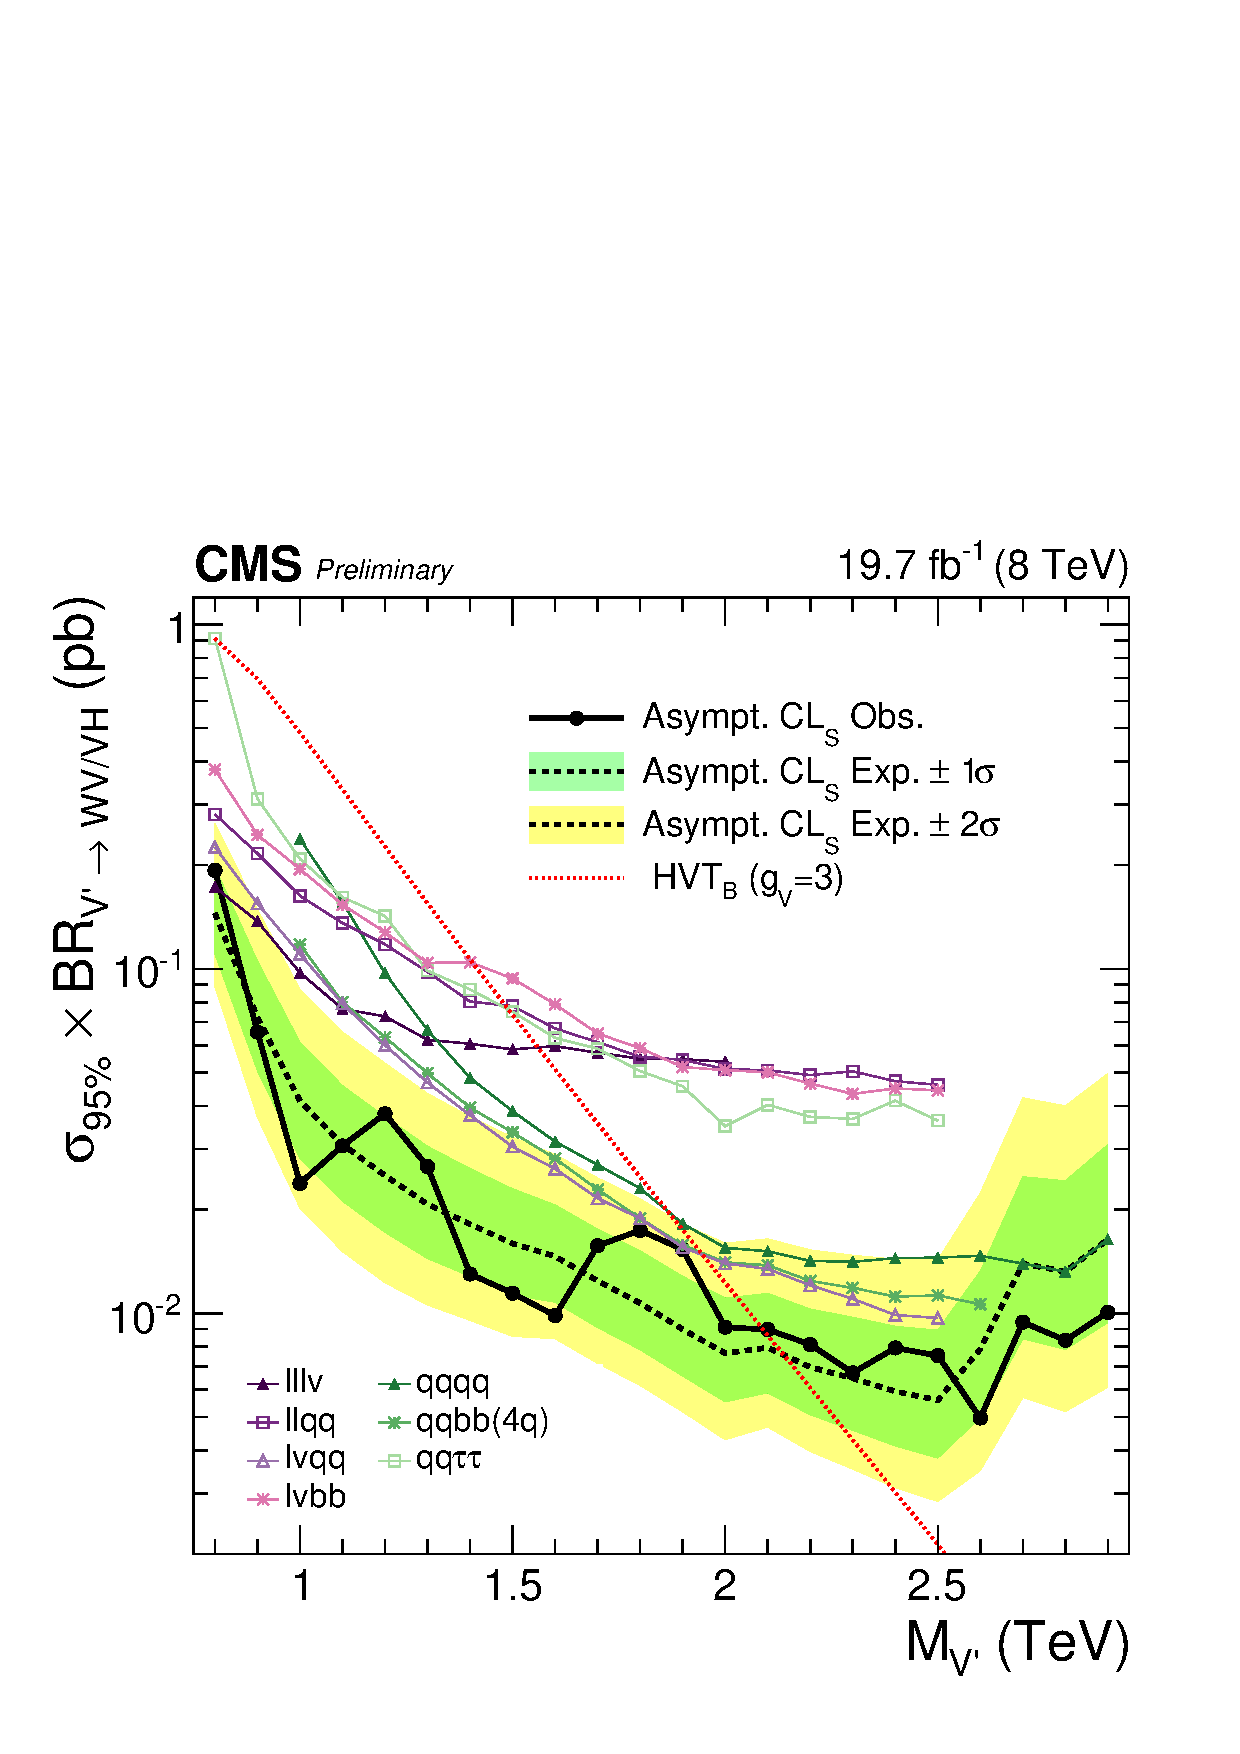
\includegraphics[width=0.48\textwidth]{\chthirteen/EXOVVhvt_compare_ALLHVT8_final.pdf}%
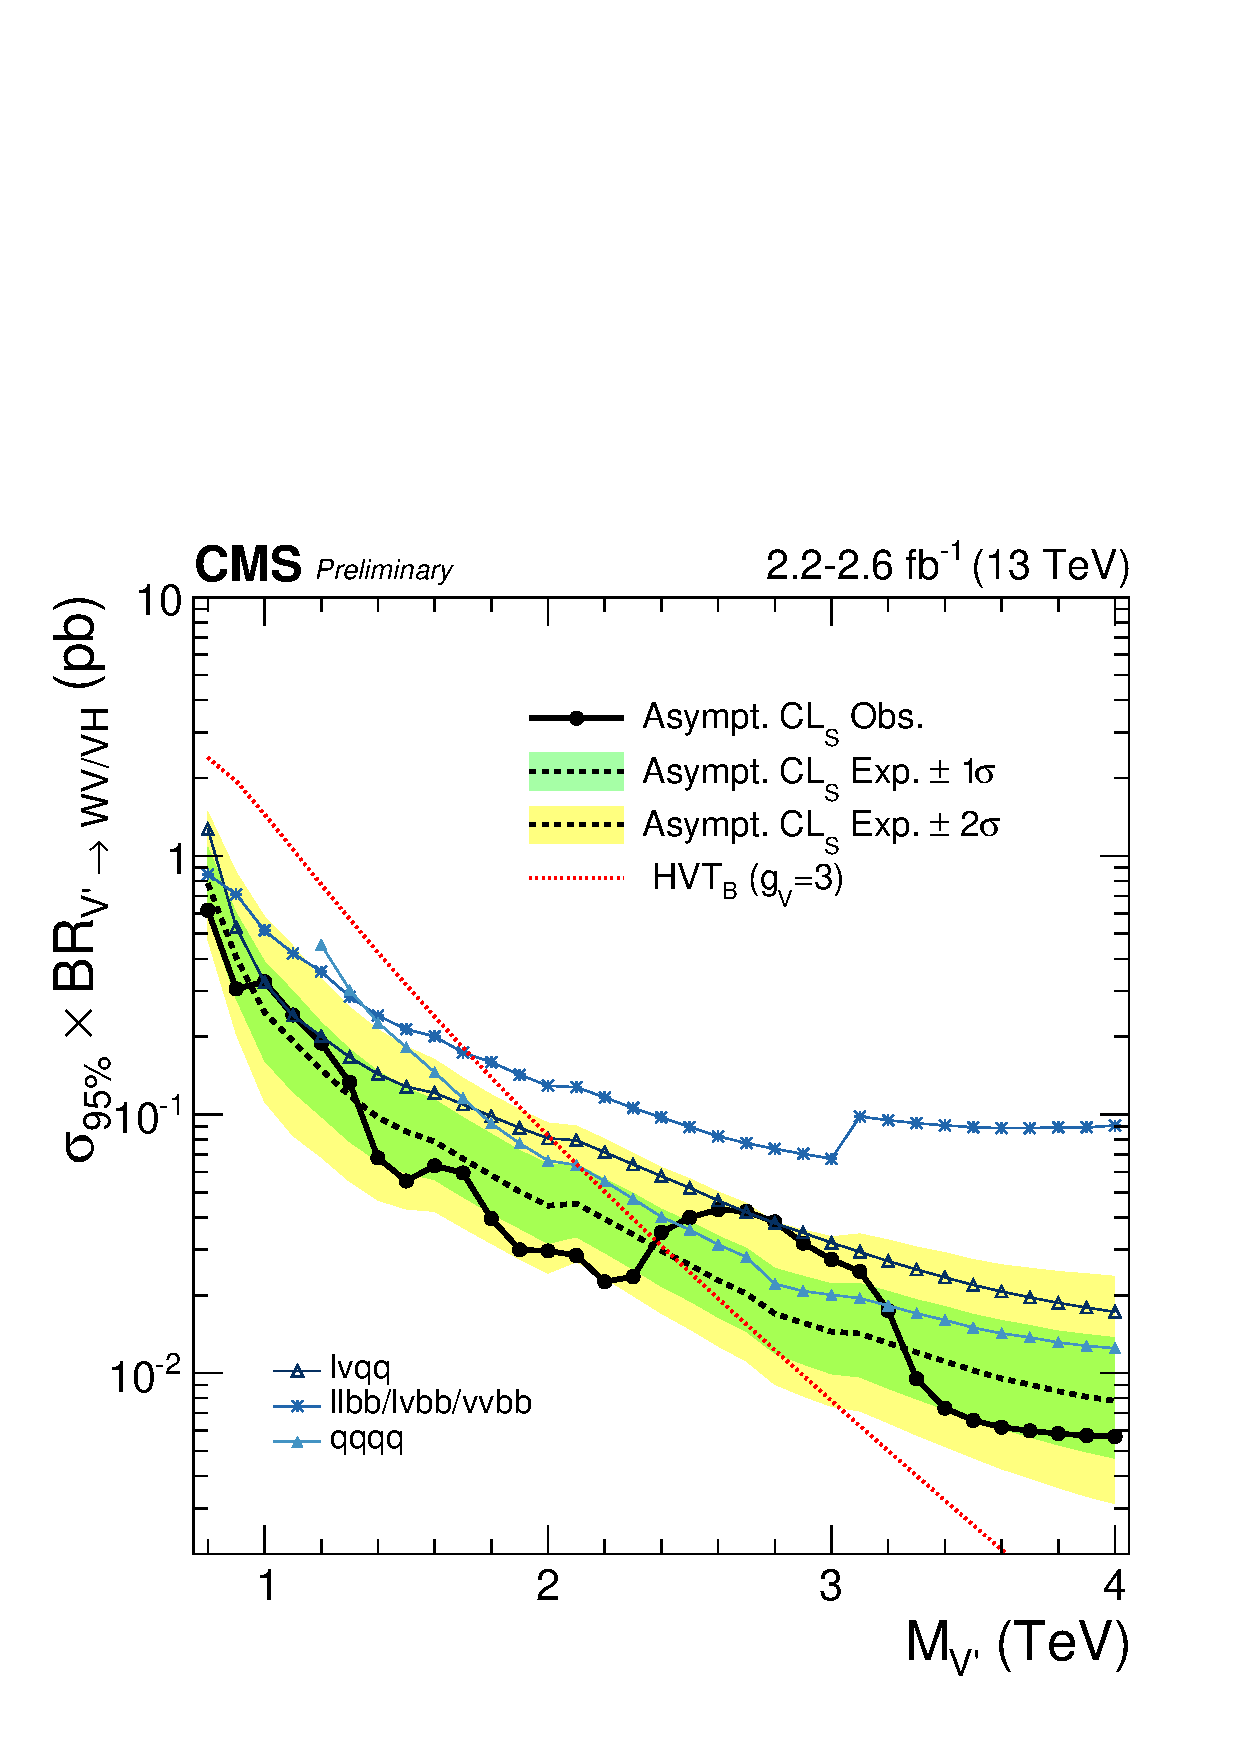
\includegraphics[width=0.48\textwidth]{\chthirteen/EXOVVhvt_compare_ALLHVT13_final.pdf} \\
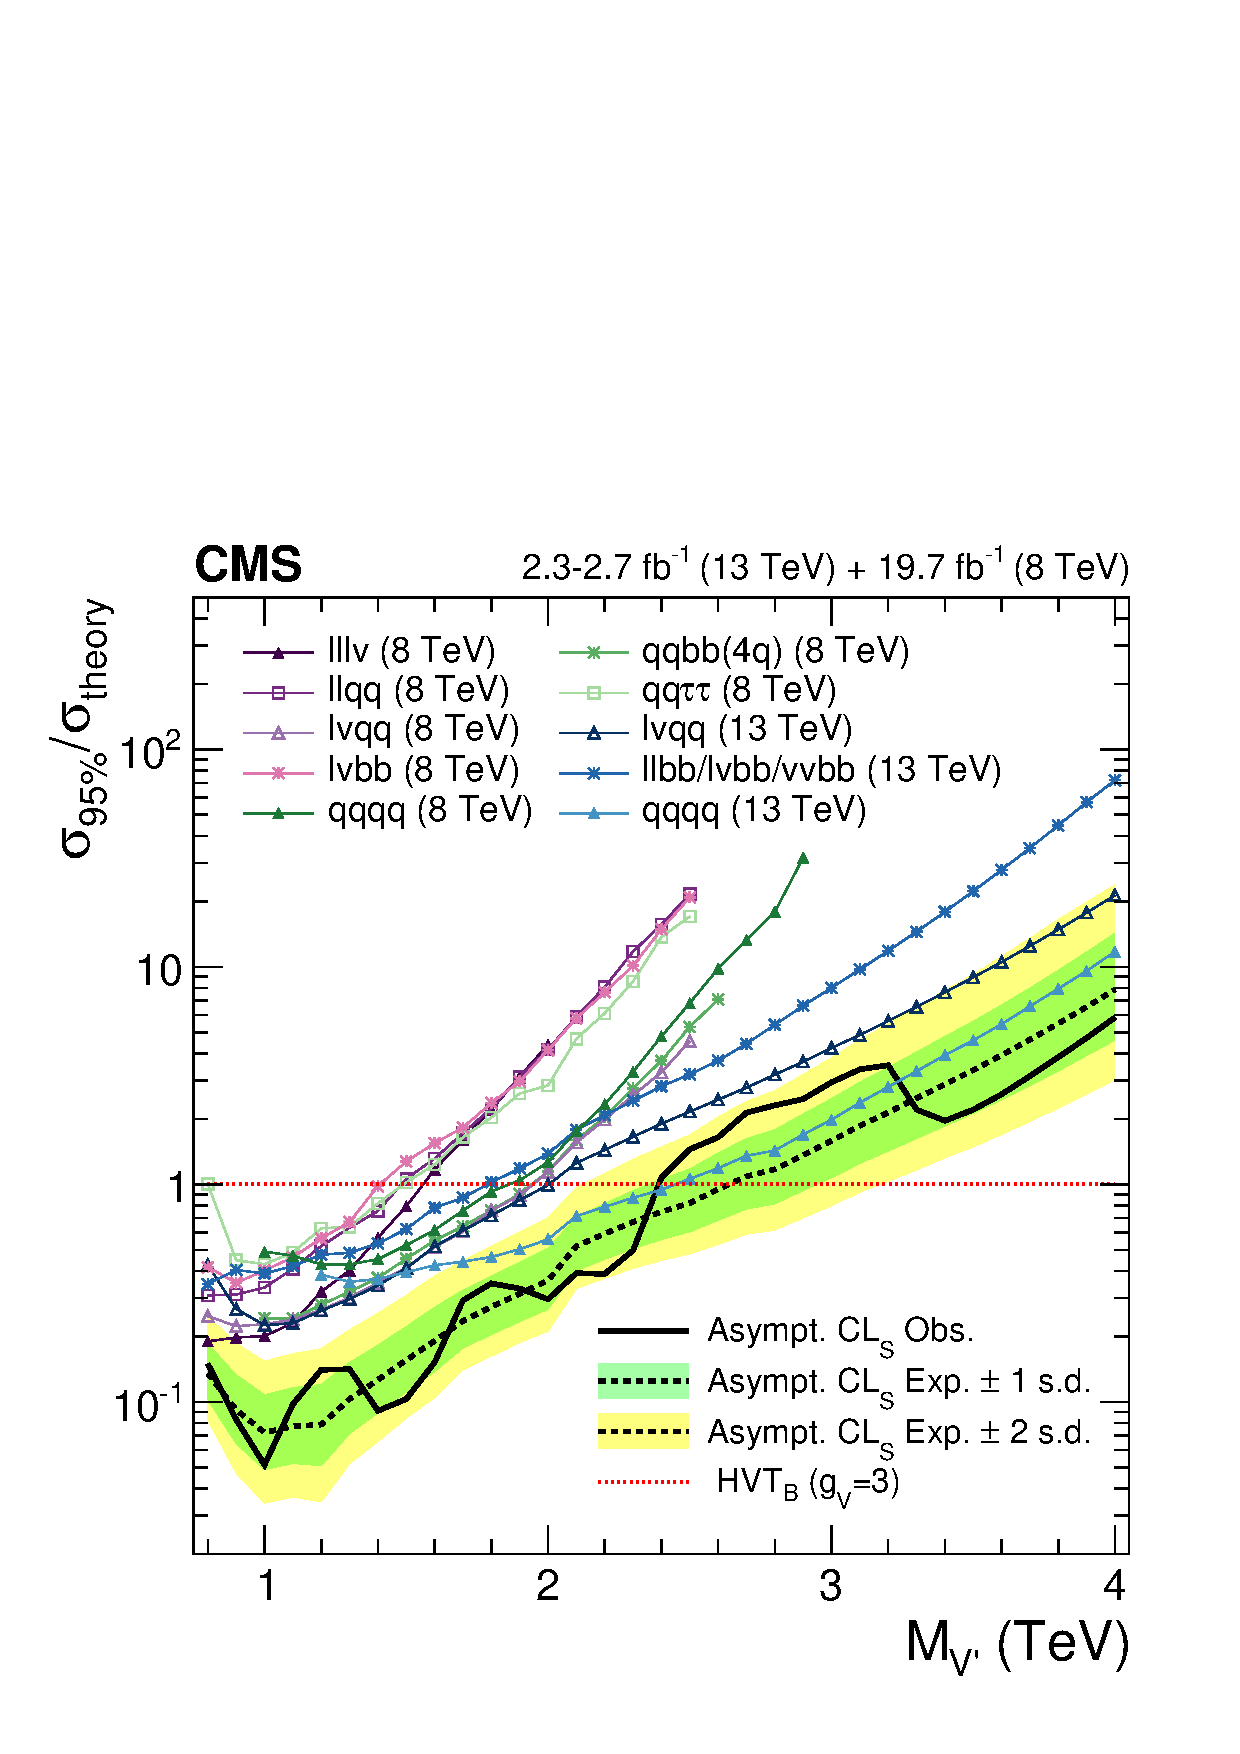
\includegraphics[width=0.48\textwidth]{\chthirteen/EXOVVhvt_compare_ALLHVT138_final.pdf}%
\caption{
(top left) Observed (black solid) and expected (black dashed) exclusion limits at 95\% CL on $\sigma( \rm pp \to \PVpr \to WV/VH)$ (\PVpr=\PWpr,\PZpr and V=W,Z) as a function of the resonance mass obtained by combining the 8 TeV diboson searches. The curve corresponding to the cross sections predicted by the HVT model B is overlaid. (top right) Observed (black solid) and expected (black dashed) exclusion limits at 95\% CL on $\sigma( \rm pp \to \PVpr \to WV/VH)$ as a function of the resonance mass obtained by combining the 13 TeV diboson searches. The curve corresponding to the cross sections predicted by the HVT model B is overlaid. (bottom) Exclusion limits at 95\% CL on the signal strength as a function of the resonance mass obtained by combining the 8 and 13 TeV diboson searches. In all the three plots the different colored lines correspond to the searches entering the combination.
}
\label{fig:hvtall_138TeV}
\end{figure}

\begin{figure}[htbp]
\centering
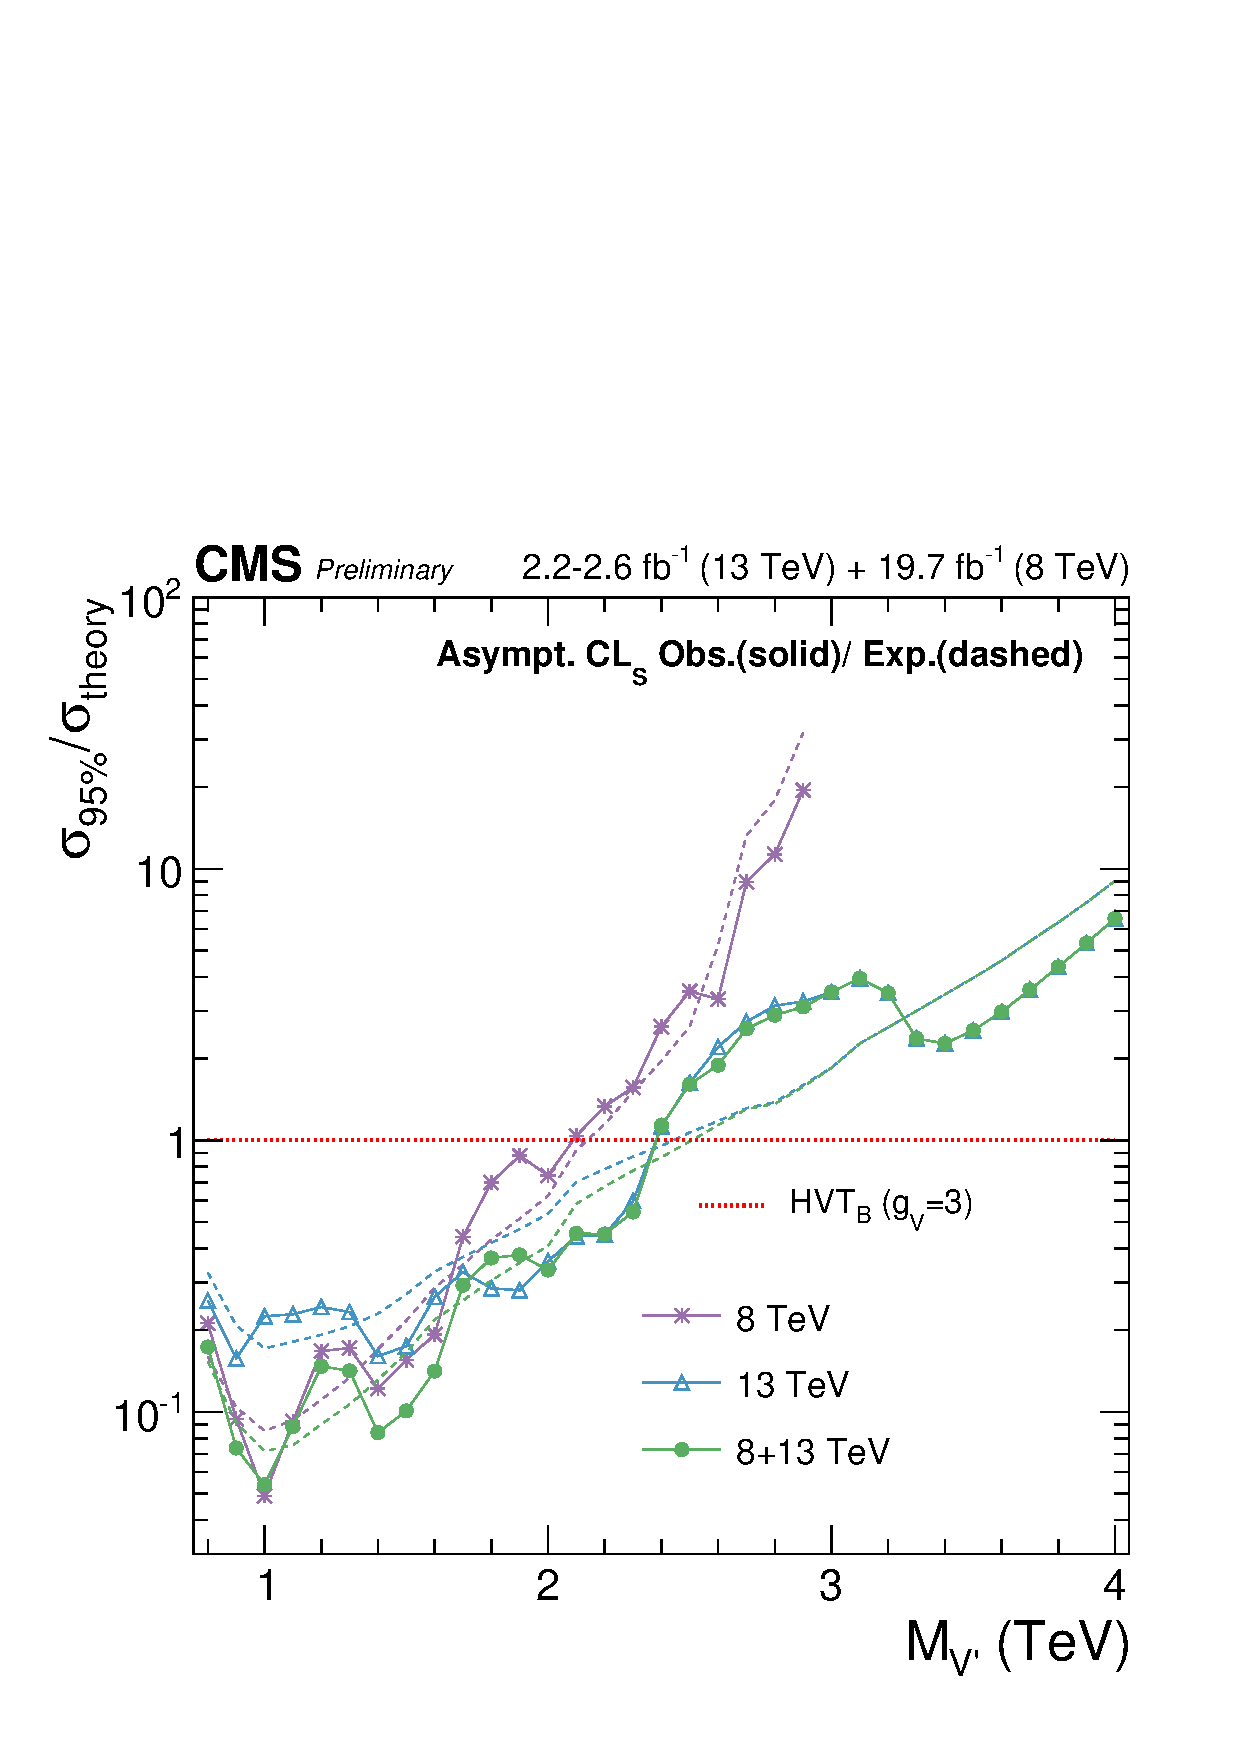
\includegraphics[width=0.48\textwidth]{\chthirteen/EXOVVhvt_compare_ALLHVT_expected.pdf}
\caption{%
Comparison of the observed (solid) and expected (dashed) exclusion limits at 95\% CL obtained by combining only 8 TeV or only 13 TeV searches to the results from the combination of all the 8 and 13 TeV results.}
\label{fig:hvtall_compare}
\end{figure}

\subsection{Limits on Bulk Graviton}

\begin{figure}[htbp]
\centering
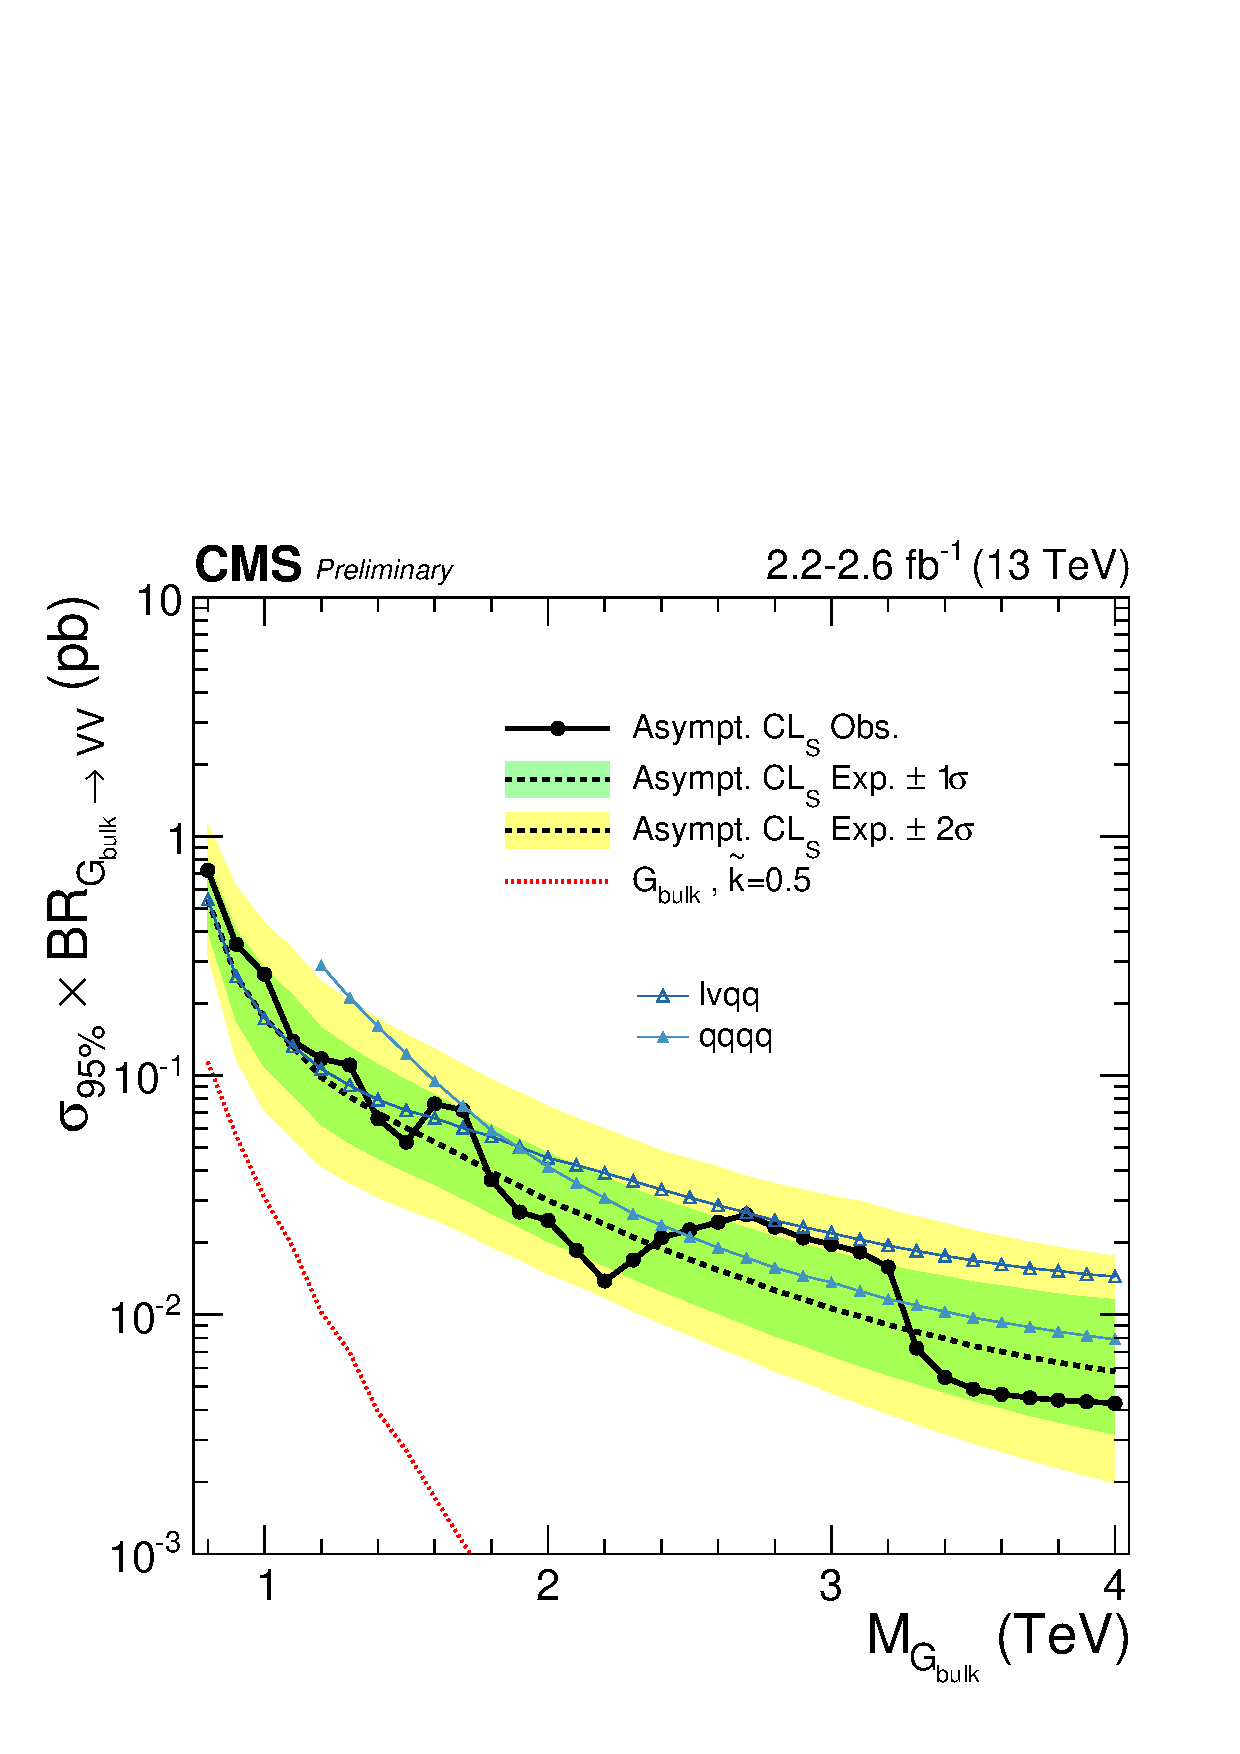
\includegraphics[width=0.48\textwidth]{\chthirteen/EXOVVbulkg_compare_ALL13_final.pdf}%
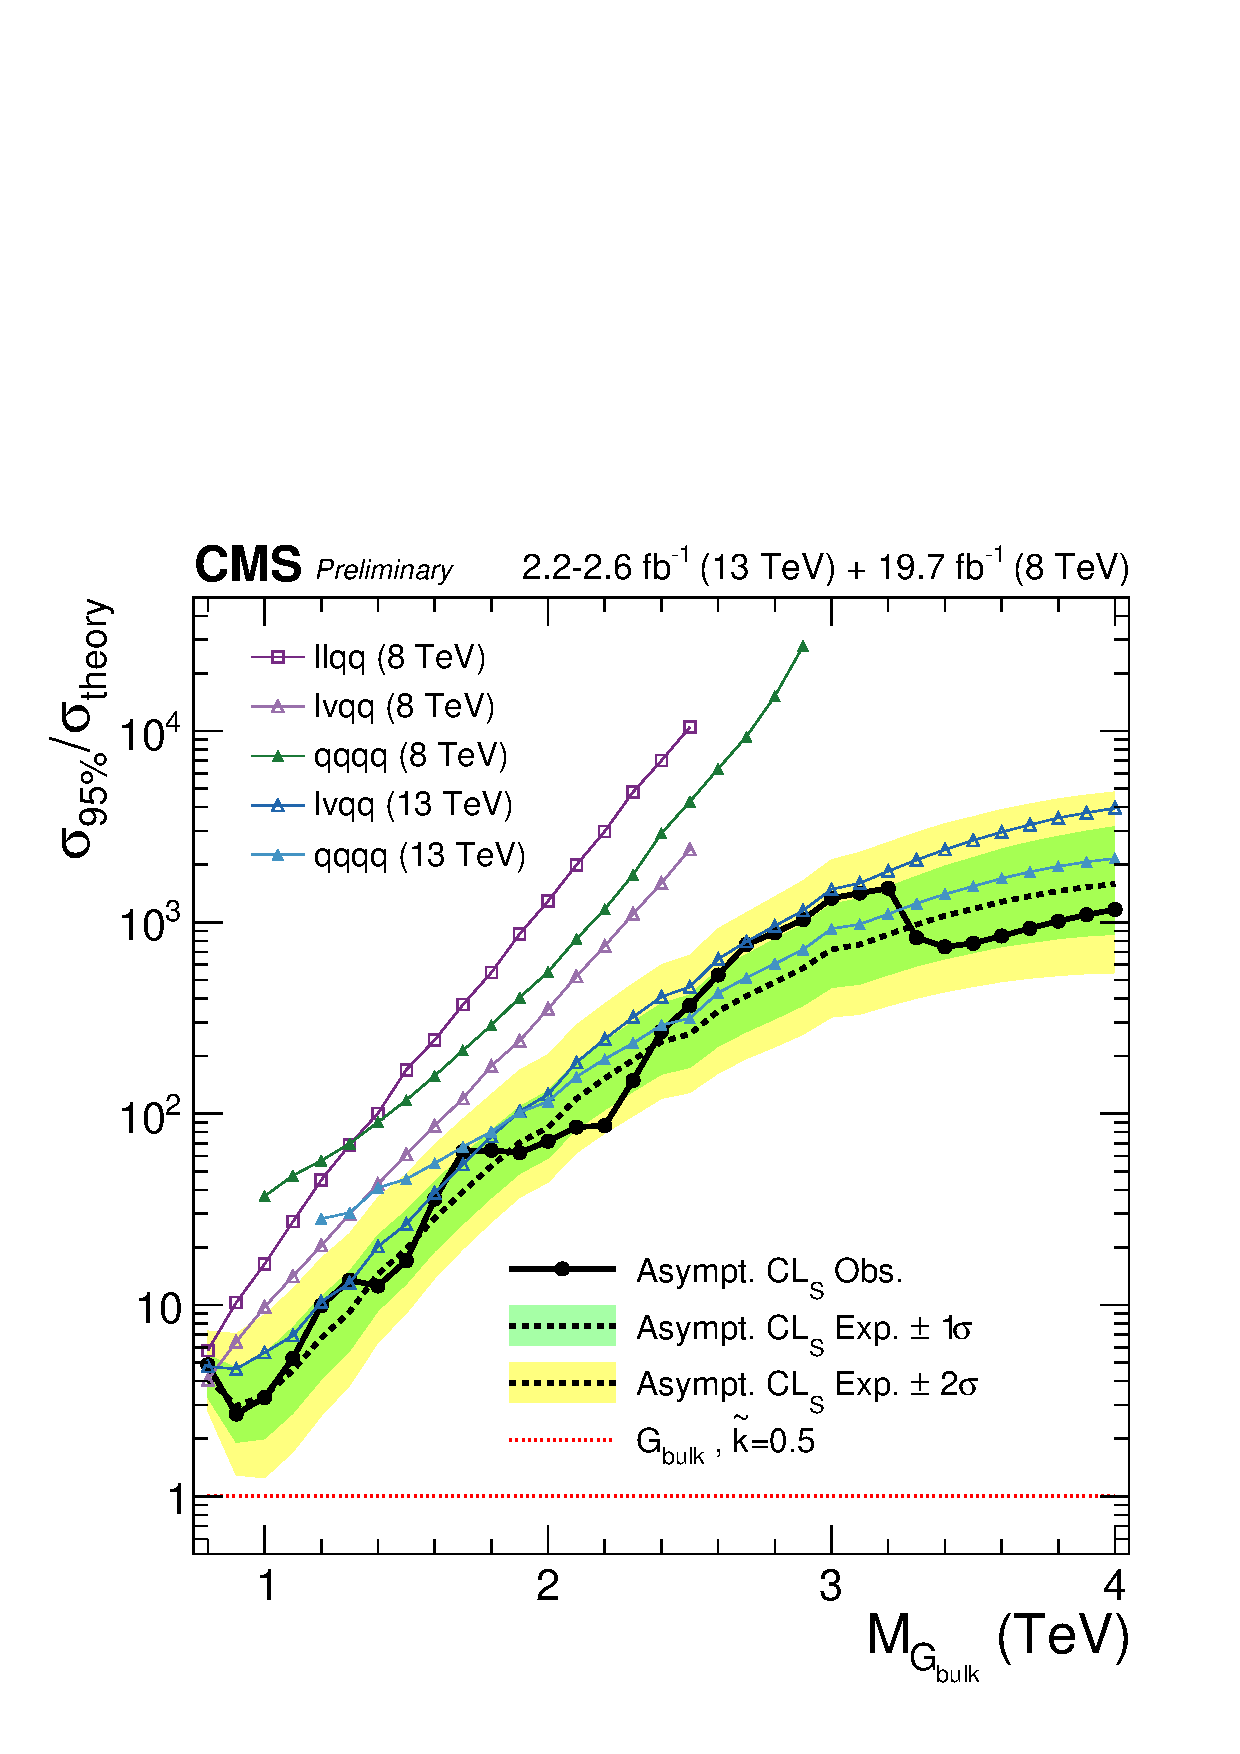
\includegraphics[width=0.48\textwidth]{\chthirteen/EXOVVbulkg_compare_ALL813_final.pdf}
\caption{
(left) Observed (black solid) and expected (black dashed) exclusion limits at 95\% CL on $\sigma( \rm pp \to G_{bulk} \to VV)$ (V=W,Z) as a function of the resonance mass obtained by combining the 13 TeV diboson searches. The curve corresponding to the cross sections predicted by bulk graviton model is overlaid. (right) Exclusion limits at 95\% CL on the signal strength as a function of the resonance mass obtained by combining the 8 and 13 TeV diboson searches. In all the three plots the different colored lines correspond to the searches entering the combination.}
\label{fig:bulkgall_138TeV}
\end{figure}

\begin{figure}[htbp]
\centering
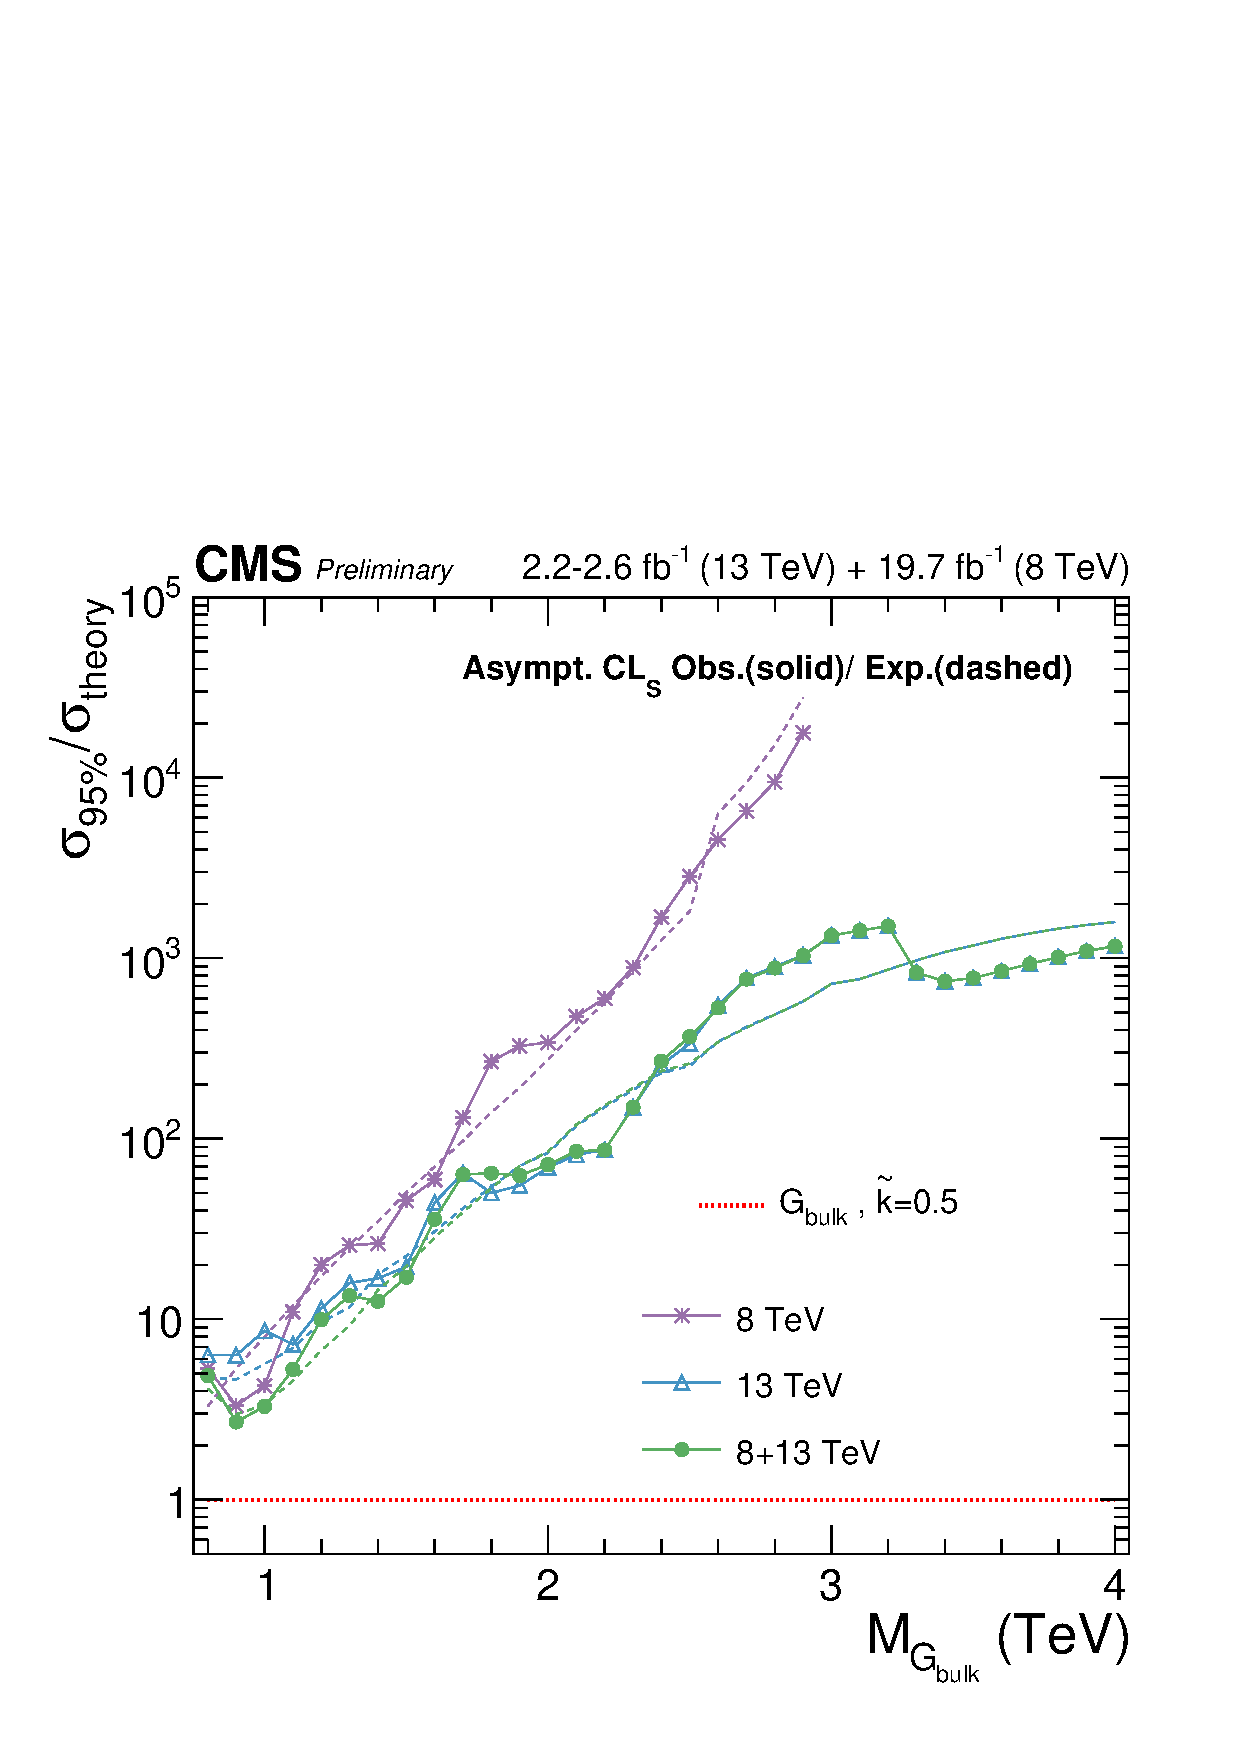
\includegraphics[width=0.48\textwidth]{\chthirteen/EXOVVbulkg_compare_ALL_expected.pdf}
\caption{%
Comparison of the observed (solid) and expected (dashed) exclusion limits at 95\% CL obtained by combining only 8 TeV or only 13 TeV searches to the results from the combination of all the 8 and 13 TeV results.}
\label{fig:bulkgall_compare}
\end{figure}

\subsection{Significance at 2 TeV}

\begin{table}[htb]
  \centering
  \caption{Statistical significance of excesses observed at 1.8 TeV in the various searches, expressed in standard deviations.}
  \begin{tabular}{l|c|c|c|c}
   Combination & \PWpr & \PZpr & HVT (\PWpr+\PZpr) & G$\rm_{bulk}$\\    
    \hline
    \hline
    VV 13 TeV             & 0.00 & 0.10 & 0.00 & 0.00 \\
    VV+VH 13 TeV      & 0.00 & 0.00 & 0.00 & - \\
    VV 8 TeV               & 1.22 & 0.56 & 1.03 & 1.61 \\
    VV 8+13 TeV         & 0.20 & 0.46 & 0.33 & 0.35 \\
    VH 8 TeV               & 2.05 & 0.56 & 1.79 & - \\
    VV+VH 8 TeV        & 2.22 & 0.77 & 1.95 & - \\
    VV+VH 8+13 TeV  & 0.86 & 0.00 & 0.83 & -
  \end{tabular}
  \label{tab:significance_1p8TeV}
\end{table}

\begin{table}[htb]
  \centering
  \caption{Statistical significance of excesses observed at 1.9 TeV in the various searches, expressed in standard deviations.}
  \begin{tabular}{l|c|c|c|c}
   Combination & \PWpr & \PZpr & HVT (\PWpr+\PZpr) & G$\rm_{bulk}$\\     
    \hline
    \hline
    VV 13 TeV             & 0.00 & 0.05 & 0.00 & 0.00 \\
    VV+VH 13 TeV      & 0.00 & 0.00 & 0.00 & -\\
    VV 8 TeV               & 1.20 & 0.46 & 0.91 & 1.05\\  
    VV 8+13 TeV         & 0.00 & 0.30 & 0.00 & 0.00\\ 
    VH 8 TeV               & 2.17 & 1.41 & 1.78 & - \\
    VV+VH 8 TeV        & 2.32 & 1.02 & 1.89 & - \\
    VV+VH 8+13 TeV  & 0.33 & 0.00 & 0.20 & -
  \end{tabular}
  \label{tab:significance_1p9TeV}
\end{table}

\begin{table}[htb]
  \centering
  \caption{Statistical significance of excesses observed at 2 TeV in the various searches, expressed in standard deviations.}
  \begin{tabular}{l|c|c|c|c}
   Combination & \PWpr & \PZpr & HVT (\PWpr+\PZpr) & G$\rm_{bulk}$\\     
    \hline
    \hline
    VV 13 TeV             & 0.00 & 0.07 & 0.00 & 0.00 \\
    VV+VH 13 TeV      & 0.00 & 0.00 & 0.00 & -\\  
    VV 8 TeV               & 0.77 & 0.75 & 0.76 & 0.44\\
    VV 8+13 TeV         & 0.23 & 0.45 & 0.29 & 0.06\\
    VH 8 TeV               & 0.00 & 0.00 & 0.00 & -\\
    VV+VH 8 TeV        & 0.58 & 0.60 & 0.48 & -\\
    VV+VH 8+13 TeV  & 0.00 & 0.00 & 0.00 & -
  \end{tabular}
  \label{tab:significance_2TeV}
\end{table}
